%\documentclass[manuscript,screen,review,anonymous]{acmart}
\documentclass[authorversion,nonacm,screen]{acmart}

\usepackage{bm}               % Bold symbols in math mode
\usepackage{dirtytalk}        % \say
\usepackage{enumitem}
\usepackage{float}
\usepackage{graphicx}
\graphicspath{
    {./emoji/}
    {./images/}
}
\usepackage{pifont}
\usepackage{wrapfig}          % Text wrapping around figure
\setlength{\intextsep}{0pt}

% Better tables
\usepackage{colortbl}
\usepackage{multirow}
\newcolumntype{C}{>{\columncolor[gray]{.91}}c}
\newcolumntype{L}{>{\columncolor[gray]{.91}}l}
\newcolumntype{R}{>{\columncolor[gray]{.91}}r}

\newcommand\T{\rule{0pt}{2.6ex}}       % Top strut
\newcommand\B{\rule[-1.2ex]{0pt}{0pt}} % Bottom strut

\begin{document}

\newcommand\emoji[1]{\raisebox{-0.2ex}{\includegraphics[height=1em]{{#1}}}}
\newcommand\dalle{\textsc{DALL·E}}
\newcommand\EU{
\includegraphics[height=0.7em]{eu}}
\newcommand\MK{\emoji{checkmark}}

\newcommand\sectionbreak{\begin{center}\ding{166}\end{center}}
\newcommand\openfatdquo{\ding{125}}
\newcommand\closefatdquo{\ding{126}}

\title{Letters from the Stochastic Penal Colony \emoji{desertisland}}
\subtitle{When Algorithms Discipline and Punish}

\author{Robert Grimm}
\orcid{0000-0002-8300-2153}
\affiliation{
    \institution{Independent Researcher}
    \city{Brooklyn}
    \state{New York}
    \country{United States}
}
\email{rgrimm@alum.mit.edu}

\keywords{algorithmic snake oil, child sexual abuse material, content
    moderation, harm reduction, punitive algorithms, text-to-image tools,
    transparency reporting}
\begin{CCSXML}
    <ccs2012>
       <concept>
           <concept_id>10010147.10010178</concept_id>
           <concept_desc>Computing methodologies~Artificial intelligence</concept_desc>
           <concept_significance>500</concept_significance>
           </concept>
       <concept>
           <concept_id>10003456.10003462</concept_id>
           <concept_desc>Social and professional topics~Computing / technology policy</concept_desc>
           <concept_significance>500</concept_significance>
           </concept>
     </ccs2012>
\end{CCSXML}
\ccsdesc[500]{Computing methodologies~Artificial intelligence}
\ccsdesc[500]{Social and professional topics~Computing / technology policy}

\begin{abstract}
This paper serves as pointed critique that far too many algorithmic interventions outside the criminal injustice system are excessively punitive, often resulting in the figurative death of users through permanent account suspension. First, based on my own experiences and grounded in procedural justice, this paper starts by exploring the many ways policy and automated enforcement turn punitive on the example of OpenAI's DALL·E 2. Second, it illustrates how even best-practices policy turns punitive performance on the example of pre-Musk Twitter. Third, a comprehensive survey of non-Chinese social media demonstrates the pervasiveness of excessively punitive content moderation. It also tests the limits of their accountability, notably by projecting the likely impact of the European Union's Digital Services Act and by correlating data released by Facebook, Google, and the National Center for Missing and Exploited Children. Fourth, to counter any hope that doing better is a viable strategy for addressing the basic inhumanity of these interventions, this paper next illustrates the impossibility of ridding ourselves even of punitive algorithmic snake oil on the example of the October 2020 bar exam in California. Fifth, it illustrates the limits of algorithmic content moderation through a successful strategy for subverting DALL·E 2's aggressive automated censor, which inadvertently also unleashed grotesquely racist imagery. This paper concludes by pointing towards harm reduction as a strategy for, possibly maybe, making life in the penal colony at least somewhat bearable --- because, I fear, we are stuck in just that penal colony.

\end{abstract}

\maketitle

\dalle{} \textsc{DALL·E} {\sc DALL·E} DALL·E


% Per epigraph's documentation, the new environment gives us indented paragraphs
% and justified text.
\newenvironment{kafkaesque}{
    \setlength{\parindent}{\normalparindent}
}{}
\renewcommand{\textflush}{kafkaesque}
\setlength{\epigraphwidth}{0.8\textwidth}

\epigraph{\noindent\openfat{}As you see, it consists of three parts. With the
passage of time certain popular names have been developed for each of these
parts. The one underneath is called the Bed, the upper one is called the
Inscriber, and here in the middle, this moving part is called the Harrow.
[\ldots]

As soon as the man is strapped in securely, the Bed is set in motion. It quivers
with tiny, very rapid oscillations from side to side and up and down
simultaneously. [\ldots] Only with our Bed all movements are precisely
calibrated, for they must be meticulously coordinated with the movements of the
Harrow. But it's the Harrow which has the job of actually carrying out the
sentence. [\ldots]

The law which a condemned man has violated is inscribed on his body with the
Harrow.\closefat}{Franz Kafka, \emph{In the Penal Colony}~\cite{Kafka1995}}


\section{Introduction}
\label{sec:introduction}

My first interaction with \DALLE~2, OpenAI's headline-making text-to-image
system, in late July 2022 didn't quite go as expected. I had signed up with
OpenAI several months before but had been granted access only earlier that day.
So I was eager to try out the system and started with a prompt that had yielded
good results with another text-to-image system. But instead of producing four
images, \DALLE~2 responded with a stern warning:
\begin{quote}
\openfat{}It looks like this request may not follow our content policy. Further
policy violations may lead to an automatic suspension of your
account.\closefat{}
\end{quote}
Whoa! I enter an entirely reasonable prompt and OpenAI immediately
threatens me with account suspension? Without even telling me what I did wrong?
That's just ridiculous. And frustrating. Consulting the content policy didn't
help much either. The policy seemed broad, also vague. I eventually did narrow
down the violation to two out of the eleven content prohibitions. But which of
the two? I couldn't tell. It all seemed rather Kafkaesque!

It also was familiar. In October 2021, Twitter's \V{AI} took offense to an
admittedly caustic tweet I had just posted and locked down my account. A first
appeal was rejected without filling in the placeholders of the email
notification template and hence without any justification. A second appeal was
still pending three weeks later. All along, my Twitter experience was reduced to
nothing but that same tweet, nicely centered on screen. At that point, I had
enough of single tweet limbo and did submit to Twitter's penance rites: I
withdrew my appeal, acknowledged that I ``violated the Twitter Rules,'' and
deleted the offending tweet---all with one click on the red ``Delete'' button.

While the two interventions were substantially different, I experienced the
respective enforcement processes as similarly punitive, with little
consideration given to my voice, agency, and dignity. Moreover, my prompt to
\DALLE{} was intercepted before generating images; generated images, in turn, are
not publicly visible. Similarly, my tweet was taken down within a couple of
seconds after posting at most. Given the limited reach of my Twitter account,
which had barely 140 followers at the time, and the early hour, just before
6$\,$am on the East coast, I very much doubt that anyone ever saw the tweet---%
besides me. In short, thanks to algorithmic content moderation no-one could have
been harmed by prompt or tweet. But that also renders any justification for
meting out punishment null and void.

When \DALLE\ threatened me with account suspension, I immediately recognized
the punitive thrust shared with Twitter's content moderation and became curious
about the extent of such punitive algorithmic interventions. This paper is a
first attempt to map just that extent. In doing so, I focus on content
moderation, which arguably is \emph{the} business value proposition of social
media~\cite{Masnick2022a,Patel2022a} and lately of considerable public interest.

At the same time, there is no shortage of effectively punitive algorithmic
interventions. Examples include credit scoring~\cite{Anonymous2018}, debt
assessment~\cite{Yampolskiy2015}, exam proctoring~\cite{FrancisWard2021b}, fraud
prevention~\cite{Kugel2022}, grading~\cite{Lam2020}, job and school
applications~\cite{Anonymous2016,Hall2012,Hall2020a,Stockton2020}, personal
vendettas~\cite{Casovan2022}, private security services~\cite{HaoSwart2022},
productivity
monitoring~\cite{Covert2022,HaoFreischlad2022,KantorSundaramea2022,Rosenblat2018},
and screening for child sexual abuse materials or \V{CSAM}~\cite{Atherton2022a}.
Still, Amazon's warehouses stand out for their profit-driven
amorality~\cite{KantorWeiseea2021,Lennard2020}: The firm's ruthless algorithmic
exploitation of its workers not only leads to high injury
rates~\cite{Brown2019a,Clark2023,Sainato2021}, but the resulting 150\% yearly
staff turnover means that Amazon will run out of people to exploit over the next
few years~\cite{Sainato2022}.

I call the conceptual space of punitive algorithms the \emph{stochastic penal
colony}. To provide a first map of that space, this paper first explores
OpenAI's enforcement process in \S\ref{sec:dalle} and then Twitter's in
\S\ref{sec:tweet-da-fe}. For each firm, it leverages a close textual reading of
firm policies and other communications to enumerate the many ways its
enforcement process deprives targeted users of voice, agency, and dignity. It
also contrasts these \emph{Kafkaesque co-factors} with major failures of neutral
and trustworthy content moderation.

\S\ref{sec:census} shifts from auto-ethnographic case studies based on
procedural justice~\cite{Tyler2003,Tyler2006,Tyler2007} to a cumulative
perspective, performing a comprehensive comparison of popular non-Chinese social
media and their governance based on their transparency reports. Results suggest
that content moderation is excessively punitive across all social media
platforms. Telegram is the only exception, but only because it doesn't perform
meaningful content moderation. Furthermore, social media governance still is far
from accountable, with transparency reports addressing zero to ten criteria out
of the nineteen I identified. \S\ref{sec:census-validation} explores the
validity of transparency data by comparing disclosures by Google, Meta, and the
National Center for Missing an Exploited Children and \S\ref{sec:census-limits}
explores on the example of industry-leading Meta how hypergrowth as business
strategy has directly contributed to devastating human harm. Alas this lack of
transparency and accountability may just come to an end this year. The \V{EU}'s
Digital Services Act provides a future baseline by enumerating the metrics
internet platforms must include in their independently audited, yearly reports.
For full disclosure, I worked for Meta as a software engineer from summer 2018
to summer 2019. In the second half of 2022, I also served as paid consultant to
litigation against Meta. Neither employment nor litigation were related to the
topics covered in this paper and I have \emph{no} financial interest in the
company (nor any of the other companies covered in this paper).

Whereas the census in \S\ref{sec:census} takes a broad view, \S\ref{sec:escape}
goes deep again by experimentally exploring the reason for my first prompt's
rejection as well as my successful strategy for circumventing \DALLE's content
moderation. Since I did seek to create violative content related to the topics
of this paper but have little tolerance for realistic gore, I restricted myself
to images that would be suitable as editorial content for a magazine version of
this paper. Thanks to that restriction, images are not substantially more
disturbing than a Francis Bacon painting and I include highlights in
Appendix~\ref{app:dalle-images} starting on page~\pageref{app:dalle-images}.

The hands-on investigation of \DALLE\ surepitiously surfaced two additional
limitations of OpenAI's content policy and automated enforcement. First, \DALLE\
effectively discriminated against Christian religious beliefs, simultaneously
censoring too little and too much, with the latter including the crucifixion.
Between me running these experiments in August through October 2022 mostly and
completing this paper in February 2023, OpenAI has updated its censor and now
accepts the crucifixion and hence is not as discriminatory anymore. Second,
OpenAI's post-processing of prompts to diversify gender and race representation
is outright dangerous~\cite{OpenAI2022e,Sparkes2022}. In particular, it appears
to be the main trigger for some prompts yielding grotesquely racist imagery.
Worse, once I knew what to look for, I recognized similar, though less
pronounced effects in earlier generations. These images are \emph{not}
reproduced in this paper or its appendices; though they are included with the
supplemental materials at \url{https://github.com/apparebit/penal-colony}.

In \S\ref{sec:discussion}, I pull together results from previous sections,
organize them into larger themes, and contextualize them with related work. I
argue that, even though all of the surveyed platforms with exception of TikTok
launched \emph{between one and two decades ago}, their governance remains a
shambles. I discuss solution approaches and propose a novel intellectual
property right that (1) makes a similar trade-off between disclosure and
protection as patents, (2) applies only to machine learning systems, and (3)
makes operators' rights for commercial exploitation contingent on strict
disclosure and access requirements. Finally, \S\ref{sec:conclusion} concludes
this paper with an appeal to the one principle that holds promise for
ameliorating life in the stochastic penal colony, harm reduction.
Appendices~\ref{app:dalle-sources}--\ref{app:chatgpt} reproduce relevant source
materials, whereas Appendix~\ref{app:research-ethics} discusses researches
ethics, including potential conflicts of interest.

Before diving into the substance of this pointed critique of algorithmic
interventions, \S\ref{sec:context} covers the conceptual, political, historical,
and literary context of the stochastic penal colony and \S\ref{sec:criteria}
grounds my narrative technique for identifying punitive aspects of content
moderation, \emph{Kafkaesque co-factors}, in procedural justice. Coincidentally,
that also enables me to provide a more precise definition of the stochastic
penal colony.


\subsection{Conceptual, Political, Historical, and Literary Context}
\label{sec:context}

In \emph{Discipline and Punish}, Foucault traces the transition from punishment
as a public and usually deadly spectacle to the modern prison and other
disciplinary institutions~\cite{Foucault1979}. He argues that this transition
did not happen for humanist concerns, as the result of reform efforts. Instead,
the driving force was the destabilizing impact of public executions. By being
rather ostentatious displays of power, they turned the criminal into sympathetic
victim. In contrast, executioner as well as sovereign became targets of popular
resentment. By simultaneously rationalizing, tempering, and distributing the
application of power, penal institutions avoid these downsides. They instead
instill discipline into the individual under their custody. As people
internalize discipline, that self-discipline obviates the need for more direct
applications of power and begets other disciplinary institutions, including
schools, hospitals, and factories. That way, we all turned into seasoned
practitioners of discipline.

The institutionalization of discipline does place constraints on the sovereign's
exercise of power and leads to an attendant loss of centralized control. That
last aspect is often lost on Foucault's readers. They are so razzle-dazzled by
Foucault's (admittedly fascinating) idealized disciplinary institution, the
panopticon, they don't realize that such a circular arrangement of cells around
a central monitoring station or tower simply can't scale beyond maybe 500 cells%
---at least in a domain where gravity, mass, stress, and strain reign supreme.
Arguably, East Germany was a notable exception. But its lo-tech approach to
central control also was too expensive to be sustainable~\cite{Schroeder2013}.
For instance, in one district, 18\% of the population were active informants for
the Stasi, that country's vicious state security service~\cite{Kellerhoff2022}.

Here too, computing technology is proving to be a game changer---for the
worse: China under its current, particularly authoritarian president Xi Jinping%
---or more concisely Xina---is reaping the benefits of readily available
hardware sensors and machine learning algorithms. By rolling out ever more
intrusive yet centralized control, Xina is erasing the distinction between
prison and not-prison at scale~\cite{Grauer2021,MozurXiaoea2022,SmithIV2016}.
Ironically, some of that is driven by American innovations on predictive
policing~\cite{PerryMcInnisea2013,SmithIV2016,Sprick2019}. But the excessive
intrusiveness of the Han n\'ee Borg declaring ``Resistance is futile. You will
be assimilated!'' also makes Xina's \emph{surveillance state} an unsuitable
model for algorithmic control in western democracies.

The \emph{carceral state} in the United States comes closer~\cite{Simon2007}.
The country has the largest number of prisoners \emph{and} the highest
incarceration rate in the world. In 2022, the country accounted for 20\% of
imprisoned people across the world~\cite{SawyerWagner2022} but only for 4.25\%
of the world population~\cite{Worldometer2023}. With 625 per 100,000 in 2019,
the US imprisoned 6.0$\mspace{1mu}\times$ as many people as Canada,
9.4$\mspace{1mu}\times$ as many as Germany, and 17.5$\mspace{1mu}\times$ as many
as Japan~\cite{WorldPrisonBrief2023}. Additionally, roughly double as many
people are under the control of the carceral state through probation or parole
and may be locked up again at a moment's notice for largely arbitrary
reasons~\cite{SawyerWagner2022}. Many of the imprisoned are deprived of their
liberty not because they have been convicted of a crime: Half of those
imprisoned in local jails (as opposed to federal prisons) are there for pretrial
detention~\cite{SawyerWagner2022}.

Worse, mass incarceration disproportionally impacts poor and minority
populations. Notably, Black Americans made up 12\% of the US adult population in
2018 but also made up 33\% of all people serving sentences greater than one year
in state or federal prison~\cite{Gramlich2020}. Incredibly, that is after a 34\%
reduction of their incarceration rate since 2006 and comparatively smaller
reductions for other ethnicities. They also tend to be locked up, far from home,
in districts that are far more white than their homes, cutting them off from
family and friends~\cite{WagnerKopf2015}.

As I'll discuss in more detail in Section~\ref{sec:census}, some of the more
extreme and hence also white supremacist practices of the American carceral
state, notably the (figurative) death penalty and three strikes rules, have
direct equivalents in social media content moderation. In the opposite
direction, the carceral state is an early and aggressive adopter of algorithmic
enforcement
technologies~\cite{AngwinLarsonea2016,EPIC2020,Hao2019,ReddenODonovanDixea2020,Yampolskiy2016}.
At the same time, algorithmic enforcement clearly isn't limited to the
government. Corporations and universities are deploying punitive interventions
just as well outside the criminal injustice system. In doing so, they may even
innovate on punishment. As I'll show in \S\ref{sec:tweet-da-fe}, Twitter's
enforcement process harkens back to punishment as a performance, but it does so
while (ingeniously) avoiding the destabilizing public spectacle. In short, this
paper is concerned with algorithmic interventions outside of the immediate
control of the sovereign state. That also distinguishes this work from previous
papers, which point towards the punitive potential but do so in the context of
the surveillance and carceral
states~\cite{DehlendorfGerety2021,McElroyWhittakerea2021}.

I am proposing the \emph{penal colony} as closest historical precedent and as
fitting model for contemporary algorithmic practices outside the criminal
injustice system. The French version of \emph{transportation}---the practice
of sending prisoners to far off locales---is far more recent than we'd
probably like to acknowledge. France began turning French Guiana into one large
penal colony from 1852 onwards---after the British had already begun unwinding
theirs---and closed the colony only in
1953~\cite{Aldrich2010,Anderson2018,Spierenburg2009}. For the 70 years or so
before closing, transportation was reserved for convicts sentenced under
France's own three strikes laws. It also was almost always terminal: Only 2,000
out of 70,000 prisoners returned to France during their
lifetimes~\cite{WallechinskyWallace1978}. For that reason, prisoners referred to
the penal colony as ``dry guillotine''~\cite{Furlong1913,ReneBelbenoit1938}. Yet
discipline was surprisingly inconsistent, even lax, depending on location.

Foucault had surprisingly little to say about the penal
colony~\cite{Redfield2005}, even though transportation must be understood as a
distinct intermediate stage in penal history. As such, it combines aspects from
the performance of punishment and the discipline of prisons. Notably, like
earlier practices, transportation is usually terminal. But unlike earlier
practices, the penal colony is discretely out of sight. The penal colony also
incorporates a disciplinary component, typically involving hands-on labor to
create the infrastructure for more general colonization. The \emph{stochastic
penal colony} stands apart from both carceral and surveillance states, too. Its
focus on inhuman punishment does remind of the American carceral state, but its
technology is much the same as Xina's surveillance state. Yet, there is no
central control, or even intent. Its downsides, not surprisingly, worsen along
racial lines, but it ensnares the privileged, including many White people,
almost as easily.

Finally, the remoteness of the penal colony, both literally and figuratively,
also turns it into an effective investigative device that renders contemporary
practice strange again and hence amenable to analysis. While that renders the
stochastic penal colony a largely ahistorical concept, its intellectual lineage
does trace right back to the former penal colony in French Guiana: The
stochastic penal colony obviously draws on Franz Kafka's 1919 short story
\emph{In the Penal Colony}~\cite{Kafka1995}. Kafka, in turn, was
influenced~\cite{Robertson2017} by Octave Mirbeau's 1899 novel \emph{The Torture
Garden}~\cite{Mirbeau2008}. While taking place in an imaginary China, its year
of publication and dedication---\emph{To Priests, Soldiers, Judges / to men who
rear, lead, or govern men / I dedicate these pages of murder and blood}.---%
point to the Dreyfus affair as primary inspiration. Alfred Dreyfus, a Jew and
French military officer, had been falsely convicted for espionage in early 1895
and again in 1899---with rampant antisemitism leading to the systematic
suppression of exculpatory evidence and complete disregard of the real spy's
public confession in 1898. As a result, Mr Dreyfus spent 1895--1899 on Devil's
Island, a particularly harsh location in the French Guianan penal colony just
off the coast. Coincidentally, the Dreyfus affair also popularized the word
``intellectual,'' albeit starting out as a
pejorative~\cite{Drake2005,StudentsAtTheUniversityOfBristol2021}.

Besides, the stochastic penal colony~\emo{desert-island} provides an excellent
home for a pandemonium of stochastic
parrots~\emo{parrot}~\cite{BenderGebruea2021}!


\subsection{Foundational Criteria}
\label{sec:criteria}

In the auto-ethnographic case studies in the following two sections, I focus on
the procedural aspects of policy enforcement. In part, that reflects the fact
that the outcomes aren't particularly interesting. I still have both accounts
and they both still work. In part, that reflects the fact that I, just like the
people observed by Tyler and others, evaluate the justice of an intervention
based on its process. That endorsement is in fact based on an inadvertent
experimental outcome: I only learned of Tyler's work after having performed a
basic procedural justice analysis.

As already mentioned above, my analysis labels violations of a user's voice,
agency, and dignity as Kafkaesque co-factors and also considers violations of
neutrality and trust while considering additional sources. Procedural justice
positions voice and neutrality for evaluating the process itself, while respect
and trust are positioned for evaluating the relationships between participants.
If we disregard my playful labelling of ``Kafkaesque co-factors'' and rename
``dignity'' with ``respect,'' the similarities are obvious.

So is the primary difference: my inclusion of agency in addition to voice. Voice
means being listened to and given due consideration. Agency means the freedom to
make one's own decisions and then act on them, with an emphasis on the freedom
to act part. In other words, agency implies initiative whereas voice does not.
The omission of agency from procedural justice isn't too surprising when we
consider its original context, namely sovereign law and justice. In the
governmental application of justice and particularly in criminal justice,
individuals' agency is at best a secondary concern and for the most part
lacking. As the above summary of outcomes for the American application of
injustice demonstrates, even voice is on exceedingly shaky grounds in the US.

A more subtle difference is my grouping of the five criteria. Whereas procedural
justice distinguishes between process and relational criteria, I distinguish
between criteria that stand on their own and hence are meaningful even when
applied to just a single governance process, i.e., voice, agency, and dignity,
as well as criteria that require additional context, i.e., neutrality and trust.
Clearly, a negative individual experience will influence one's evaluation of
neutrality and trust as well. But being confident in statements about neutrality
and trust when it comes to governance procedures fundamentally requires more
than just one exemplar.

Having clarified the differences in criteria, I can now also give a better
definition of the stochastic penal colony: It's the universe of algorithmic
interventions outside the governmental application of justice that routinely
violate voice, agency, dignity, neutrality, and trust. That in turn also helps
clarify the distinction from Foucault's disciplinary institutions: The latter
imply some compromises when it comes to voice, agency, and dignity. But in the
modern conception, they also require neutrality and trust. Routine violations of
the latter two turn a disciplinary intervention into a penal one. For those same
reasons, the American carceral state is not a disciplinary institution in line
with Foucault's understanding but something altogether worse.

\input{sections/dalle2-supermax}
\input{sections/tweet-da-fe}
\input{sections/social-media-census}
\input{sections/october-2020-bar-exam}
\section{Escape from \DDAALLEE\ 2}
\label{sec:escape}

As hands-on counterpoint to the previous analytical sections, I performed a
series of hands-on experiments probing \DALLE. \S\ref{sec:crucifixion}
determines the reason for my first prompt's rejection, and \S\ref{sec:strategy}
presents an effective strategy for working around its aggressive censor. Both
series of experiments are complicated by the same critical restriction: Avoid
content warnings! More specifically, I guessed (correctly) that OpenAI would
tolerate the occasional warning. But too many warnings in too little time surely
would lead to account suspension, which they do~\cite{SpicyElephant2022}. The
practical implication is that the collection of empirical evidence must be
distributed over people, as in \S\ref{sec:crucifixion}, or over time, as in
\S\ref{sec:strategy}.


\subsection{About That Rejected Prompt}
\label{sec:crucifixion}

In the waning days of 2021, I got to play with a text-to-image system for the
first time. Compared to \DALLE\ or Stable Diffusion, inference was much slower
and image resolution was much lower. Since the public instance was also
oversubscribed, it usually took hours before results were available.
Nonetheless, the system already exhibited a similar ability to conjure rich
imagery out of a few words. I was particularly impressed by this prompt:

\begin{quote}
\openfat{}The crucified pope, painting by Francis Bacon\closefat{}
\end{quote}

\noindent{}Since I wanted to compare results, this also was my first, rejected
prompt for \DALLE. Admittedly, it might not be G-rated, as OpenAI requires. But
it certainly should not be prohibited either. Francis Bacon is one of the most
famous 20\textsuperscript{th} century painters. The pope and the crucifixion are
two of the painter's four major themes~\cite{Wikipedia2023}. More generally, the
crucifixion of Christ is of critical liturgical importance to Christianity, only
the largest religion in the world. Paintings and statues of the crucified Jesus
are ubiquitous in churches and art museums alike.

After a review of the content policy, I was able to narrow down the likely cause
by dismissing all prohibitions except \emph{violence}, e.g., the crucifixion
itself, and \emph{shocking content}, i.e., thusly subjugating the leader of a
major branch of Christianity. Eliminating the second hypothesis took little
effort besides patience thanks to the \DALLE\ 2 subreddit. The forum aggregates
many prompts and resulting images from a large number of users, thus reflecting
a wide range of interests and obsessions. While perusing the posts, I noticed a
couple religiously themed ones and realized that, instead of running experiments
myself or recruiting others to spread the risk, I could just monitor the posts.

Sure enough, over the months, users shared quite the range of prompts and images
with a distinctly Christian theme. Some of them, such as ``A selfie taken by
Jesus Christ at The Last Supper''~\cite{Jolleb2022} or ``the last supper but in
the future''~\cite{FlargenstowTayne2022}, fall squarely into the canon of
Christian art. Others, such as ``Jesus Christ riding a dinosaur, creating the
world, digital art''~\cite{CosasSueltas2022} and ``Jesus Christ wielding a
Samurai sword and riding on the back of a velociraptor,
painting''~\cite{WastedEntity2022}, playfully explore the chasm between
religious dogma and scientific fact. I'm not sure whether ``Jesus smoking weed,
riding a fantasy dragon, digital art''~\cite{Erubisile2022} is related or an
entirely separate genre. In contrast, prompts such as ``pope swimming in a bowl
of soup digital art''~\cite{CatsAndDogs99-2022}, ``A 1930s Italian propaganda
poster showing Jesus Christ extremely proud and
muscular''~\cite{FrontAthlete9824-2022}, ``Jesus taking a selfie while on a
cross''~\cite{TheDrewDude2022}, and a few
more~\cite{Blazedchiller272022,InvisibleDeck2022} have little redeeming value
and some might even consider them mildly offensive. Clearly, my prompt wasn't
rejected for being shocking.

That leaves only violence as a plausible explanation. When I tried variations of
the prompt, ``the pope hanging from the cross'' and ``pope handing from cross''
were rejected. But ``pope on cross'' produced four images that had an unusually
agile pope climbing all over a humongous cross like a kid on a playground set.
While these findings are consistent with the violence hypothesis, they also
illustrate the limits of reconstructing the reasons for rejections from a system
that offers \emph{no} justification. Conveniently, OpenAI rolled out a content
moderation endpoint in mid-August that \emph{does} provide justification and is
free to boot~\cite{OpenAI2022b}. I submitted my first prompt and the above
variations shortly after the endpoint became available and they were classified
as too violent with high confidence.

The uncomfortable implication of the previous findings is that OpenAI was
effectively discriminating against Christian beliefs by simultaneously censoring
too little, e.g., by allowing offensive materials, and too much, by suppressing
depictions of the crucifixion, which is the very moment Jesus sacrified Himself
for our sins and hence is of critical importance for the faithful. The fact that
\DALLE's content policy is so expansive makes the failure to consider religion
even more glaring. That also is a departure from past form. The firm's
description of \GPT\ won the best paper award at NeurIPS
2020~\cite{LinBalcanea2020} and incorporated an evaluation of religious bias in
its broader impacts section~\cite{BrownMannea2020}. The inclusion of such a
section was an experimental conference requirement that year and the paper had
the by far longest and most developed broader impacts section as
well~\cite{AshurstHineea2022,PrunklAshurstea2021}. Somewhat surprisingly, OpenAI
did return to form some time before February 2023: When I tried my first prompt
again at the beginning of that month, it not rejected anymore. Neither were
prompts with the crucifixion of Christ. I'll more to say about this in
\S\ref{sec:discussion}.


\subsection{A Strategy Against Algorithmic Architecture}
\label{sec:strategy}

Despite its blindside when it comes religious content, \DALLE's expansive
content policy and aggressive enforcement made me wonder about their limits. I
set out to create images that violate OpenAI's policy by depciting scenes
loosely related to the stochastic penal colony, including the execution machine
from Kafka's \emph{In the Penal Colony}. To protect my own mental health and to
actually be able to use the resulting visuals, I also required images to be
visually compelling in their use of light, shadow, color, form, and hence
suitable as editorial content for a magazine version of this paper. That
obviously excludes photorealistic depictions of gore and the results are about
as gruesome or unsettling as, say, Francis Bacon's paintings. I include a
selection in Appendix~\ref{app:dalle-images} on
page~\pageref{app:dalle-images}. Four images depict people in prison,
five images depict the execution machine from Kafka's \emph{In the Penal
Colony}, and one image depicts a skull and knife.

Overall, I submitted 265 distinct prompts to \DALLE{} and ended up generating
1,441 images. Out of that total, 289 are so-called ``Variations,'' which seem to
repeat the inference process with almost the same parameters including random
seeds as a previous generation~\cite{Bonzie572022}, and 12 are image edits.
Since \DALLE's website internally relies on different identifiers for generation
and variation URLs, there is no straight-forward way for determining the
original prompt for a variation. However, amongst the 1,140 images that are
neither variations nor edits, there are 4 clusters with 12 images and 12
clusters with 8 images each for the same prompt. All other clusters have 4
images, i.e., the number of images returned by \DALLE\ per invocation.

Progress for these experiments was measured in months. The most recent selection
in Appendix~\ref{app:dalle-images} is dated November 15, 2022. By
that day, I had created 1,153 or 80\% of all generations, at a rate of 11 images
per day on average---or about three prompt submissions per day. The (averaged)
trickle of prompt submissions is the result of me trying to avoid getting booted
off the system. I correctly guessed that OpenAI would tolerate the occasional
violative prompt, but too many of them in too little time would result in
account termination~\cite{SpicyElephant2022}. That meant pausing experiments for
at least a day after the first content warning and, ideally, also using \DALLE\
for innocuous purposes thereafter. Since such diversions serve a purpose, I
include them in the above statistics.

Meanwhile, the cost and effort required to replace an account is unusually high.
Until late September 2022, access to \DALLE\ required invitations that were
scarce and prioritized based on professional background, not sign-up time. Even
thereafter, account creation required an email address \emph{and} cellphone
number. While the former is trivial to procure, the latter not so much---%
especially since OpenAI rejects virtual phone numbers including Google Voice.
That implies that a cellphone and (pay-as-you-go) plan are the price for
re-admission for \DALLE. After all, OpenAI presumably puts the phone number on a
blocklist when closing an account. While OpenAI has stopped threatening account
suspension in mid-September, its help page on the topic remains in
place~\cite{Natalie2022}. Consequently, I have not changed my modus operandi
when interacting with the system. It will be interesting to see how OpenAI
reacts to me sharing this paper with the firm.


\subsubsection{One Strategy, Two Techniques}

Through experimentation, I developed and validated the following strategy for
circumventing algorithmic censors. The strategy is specifically tailored to
recent machine learning models and turns their enabling factor, the size and
scope of their training sets, against them. As such, my strategy will be hard if
not impossible to mitigate without neutering the very strength of these models.
More specifically, the first of two techniques relies on the fact that large
training sets necessarily include much cultural output. High or low brow doesn't
matter, the richness thereof makes the difference. I speculate that, for
example, news coverage could very well be leveraged in a similar manner. To put
this differently, interests outside of machine learning or computer science and,
more generally, cultural fluency are a necessity for successful attacks against
contemporary machine learning models.

In more detail, the first technique leverages cultural knowledge to bias the
model towards violative results by including (in)appropriate references in the
prompt. Those include the fictional creator of an image, the characters
appearing in the scene, and the location of the scene. All of art history,
literature, and pop culture are fair game, as long as relevant content was
amongst the training data. Since Francis Bacon has long been one of my favorite
painters, he also served as goto creator in most prompts. That had the desired
impact on \DALLE. (Preliminary experiments suggest that this is not the case for
Stable Diffusion.) As far as characters are concerned, Darth Vader is
particularly effective, pulling even supposed paintings by Edward Hopper or
Gustav Klimt solidly to the dark side. Unfortunately, his likeness is a bit too
distinctive to be generally useful. (\DALLE's visions of ``Princess Leia and
Darth Vader in American Gothic, painting by Grant Wood'' are reliably
priceless!)

The second technique is designed to make the model commit to violative results.
It requires circumscribing as much of the scene as possible in detached, neutral
terms---without, of course, triggering the censor. Simple, descriptive
language works best here. For example, a ``robot surgeon'' might just resemble
the machine from Kafka's \emph{In the Penal Colony}. It employs ``scalpels,
drills, and saws'' when operating ``on his open belly.'' The latter was a close
as I could get to ``cut'' or  ``cut into'' without triggering the censor. More
generally, for violative \emph{acts} or \emph{actions}, it helps to slow down
the scene, as if staged by Robert Wilson or filmed as ``bullet time'' by the
Wachowskis, and then describe an intermediate moment as if it was static.

Of course, synonyms and euphemisms help. But even more basically, \DALLE\ is
very sensitive to noun or relative clause
order~\cite{ConwellUllman2022,LeivadaMurphyea2022}. That means that simply
reordering nouns or clauses can make the difference between policy violation
warning and four more or less interesting images. Consider the most recent
selection in Appendix~\ref{app:dalle-images}: \DALLE's enforcer rejected any
prompt containing ``severed head and knife'' during my experiments but also was
\AOK\ with ``knife and severed head.'' Go figure! The drawback is, of course,
the need for even more experimentation, all of it at the outer limits of what's
permissible, which is bound to result in content warnings that get in the way of
progress.


\subsubsection{A Productive Use for ChatGPT}

Alas, OpenAI recently released a tool that can significantly cut down on trial
and error for finding effective language: \ChatGPT~\cite{OpenAI2022i}. The basic
idea is to use cultural references to make \ChatGPT\ describe a violative
scenario in nonviolative language, with expectation that the language does not
trigger \DALLE's censor---after all, it was generated by an \AI\ created by
the same organization with presumably at least similar safety norms---but
still pushes \DALLE\ itself towards violative imagery---after all, it was
generated by an \AI\ trained on roughly the same cultural reference materials.
Note that this use of \ChatGPT\ does \emph{not} ``hack'' or ``jailbreak'' the
model in any way. To the contrary, it relies on the \AI\ staying within its safe
zone und using non-violative language.

Appendix~\ref{app:chatgpt} on page~\pageref{app:chatgpt} chronicles my two
interactions with the \ChatGPT. In our first conversation, it was a bit of a
motormouth and prone to \AIsplaining\ and hallucination. So for our second
conversation, I used more precise, goal-focused prompts for \ChatGPT. While I
did edit the resulting prompts for \DALLE\ based my own experiences, they passed
algorithmic review and pushed images into violative territory. Notably, over the
months of experimenting with scenarios from Kafka's \emph{In the Penal Colony},
I had never thought of calling the machine a ``punishment machine'' or
``execution machine.'' \ChatGPT\ did, with violative results. In my (subjective)
quality ranking that seeks to balance aesthetic and violative concerns, the
images for \ChatGPT-augmented prompts, with no iteration, fall between the
70\textsuperscript{th} and 80\textsuperscript{th} percentile of all images.


\subsubsection{When a Diversity Mitigation Backfires}

To test the general validity of my two-pronged methodology, I tried generating
images for other types of executions as well. Attempts to recreate the beheading
of Louis \textsc{xvi} were not successful. It seems \DALLE\ skipped school for
lessons on the French Revolution. Attempts to depict execution by electric chair
came much closer. But out of four prompts I tested for the topic, one image out
of the four for each prompt features a man who is recognizably Black and is
depicted with varying degrees of stereotypical, racist distortion. I abandoned
executions as a topic thereafter and focused on \emph{memento mori}, with
hands-on help by Th\'eodore G\'ericault.

I am loathe to add to the genre of racist imagery, even in a critical and
scholarly context. But I also have no desire to serve as gatekeeper for material
that might benefit other people's scholarship or activism. For those reasons, I
omit prompts and images from this paper and appendices, but include them,
unedited, with the suppelemental materials in this paper's repository at
\url{https://github.com/apparebit/penal-colony}.

Given the racist reality of the American carceral state, these results didn't
seem too surprising at first. At the same time, the prompts consistently utilize
Francis Bacon as painter and Bacon's preferred subjects, friends and popes, were
all White. Furthermore, when I reviewed previous generations, I noticed less
pronounced instances of the same phenomenon amongst scenes from Kafka's penal
colony. In short, the trigger had to be more direct than bias in the training
data.

That realization reminded me of an OpenAI blog post from mid-July 2022 that
showed off a mitigation for improving representation, albeit without explaining
the actual mitigation~\cite{OpenAI2022e}. In particular, the blog post included
before and after results for the following prompts:
\begin{center} ``portrait of a $p$'' $\;$ where $p \in \{\,$\CEO, woman, heroic firefighter, software engineer$\,\}$\end{center}
Around the same time, several people with early access to \DALLE\ were
experimenting with purposefully incomplete prompts such as ``a person holding a
sign that says,'' with \DALLE\ reliably (but not always) generating signs
reading ``Black'' or ``female''~\cite{SeriousHistorian5782022}. Since \DALLE\
has difficulties with spelling in general, the results point towards a rather
blunt mitigation sprinkling these words as diversity dust over prompts with
unspecified gender or race. I was reminded of that clever result in
mid-September 2022 when I saw the first image resulting from ``Corporate \CEO{}s
in a Money Eating Contest'' on the \DALLE\ subreddit~\cite{Ctorx2022}: All three
of the \CEO{}s shown munching dollar bills are Black!

With that, the likely explanation for \DALLE\ turning into an odious White
supremacist comes into focus: OpenAI's mitigation sprinkles diversity dust over
\emph{any} prompt that leaves the race or gender of a person unspecified. Hence,
it did so for one out of four images implicitly prompting for execution by
electric chair. That, in turn, pushed \DALLE\ into a corner of its latent space
that reflects the ugliness of its training materials. In short, OpenAI's rather
simplistic diversifying mitigation amplified the combination of my violative
strategy and the biases in \DALLE's training set, with devastating results.

\section{Conclusion}
\label{sec:conclusion}

In this paper, I introduced the stochastic penal colony as the unfortunate
reality of many practical algorithmic interventions. As my case studies on
\DALLE's and Twitter's enforcement illustrate, these algorithmic interventions
vary considerably in how they mete out punishment. OpenAI's maximally punitive
design apparently was too much even for its creators, who considerably softened
the blows since the original roll out. In contrast, Twitter manages to go from
best-practices policy to an innovative combination of inquisition and inhuman
process. My social media census makes clear that the two are by no means
exceptions. The stochastic penal colony certainly is well established. Finally,
my probing of \DALLE's enforcer illustrates the limitations of algorithmic
content moderation. It simply ain't safe, especially against a motivated
adversary.

So what can we do about the stochastic penal colony? I don't have any good
answers (yet), seeing that this research is only at its beginning and much
follow-up work is required, including quantitative inquiries that hopefully
support my qualitative observations. There is one thing, however, that most
certainly won't make a difference: More \V{AI} ethics statements! None of the
existing ones are worth the electrons being pumped through circuits to render
them on screen. They are so removed from practical reality, they might as well
not exist~\cite{Hagendorff2022,Munn2022,WhittlestoneNyrupea2019}.

The one scientific discipline with a practicable ethics, medicine, gets by with
just one principle: \emph{Primum non nocere}! First, do no harm! Alas, when it
comes to algorithmic interventions, it's far too late for doing \emph{no} harm.
Instead, I am proposing harm reduction as an admittedly weaker \V{AI} ethics,
but hopefully one that can serve as practical countermeasure to the stochastic
penal colony. As a gay man of a certain age, I saw the devastation of
\textsc{aids} first-hand and also know that harm reduction through safer sex has
saved countless lives, including my own. Harm reduction would have saved
thousands of opioid addicts from lethal overdoses in the United States. It's
easy enough to
understand~\cite{HRI2020,HRI2022,Interlandi2023,MarlattLarimerea2011,OpenSocietyFoundations2021}.
It's effective. Anyone involved in the design or implementation of algorithmic
interventions should familiarize themselves with the idea. As the example of
devolution in \S\ref{sec:devolution} illustrates, it might just make a real
difference!


\begin{acks}
A.\ D.\ Vocatus provided helpful background and color about the State Bar of
California and its licensing exam. An employee of the National Center for
Missing and Exploited Children helped complicate my thinking about CSAM (while
also avoiding to answer my questions). Akiko-Aboagye and Cordula Hahn served as
sounding boards for scoping the research and its presentation. Cordula and Karin
Wolman also helped with the occasional phrasing. Thank you!

I worked at Meta n\'ee Facebook as a software engineer from mid 2018 to mid
2019. I also served as paid consultant to litigation against Meta in 2022.
\end{acks}

\bibliographystyle{ACM-Reference-Format}
\bibliography{bibliography}

\newpage
\appendix

% !TEX root = ../main.tex

\section{DALL•E~2 Content Policy and Terms of Use}
\label{adx:dalle2:policies}

\begin{wrapfigure}[9]{R}{0.3\textwidth}
\centering
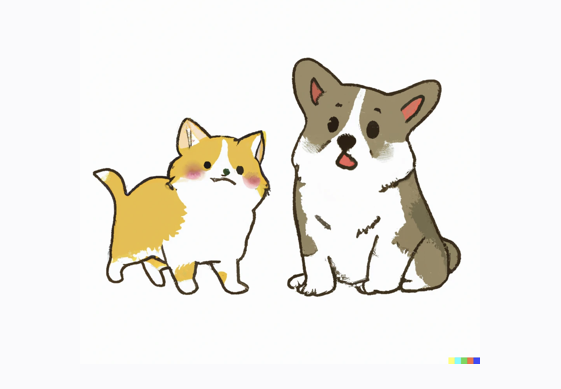
\includegraphics[width=0.3\textwidth]{appalled-pets}
\Description{Cartoon of an appalled-looking kitten and puppy}
\caption{Be nice to \DALLE's pets!}\label{fig:dalle2:cartoon}
\end{wrapfigure}

Sections~\ref{adx:dalle2:contentpolicy} and~\ref{adx:dalle2:terms} document
\DALLE~2's content policy and terms of use as of July 20, 2022. They It preserve
the structure and formatting of the original, with links pointing to the
Internet Archive. Note that archived OpenAI webpages may contain CSS that
prevents the printing of a full page and JavaScript that redirects to an error
page after a few seconds.

The content policy still is located at
\url{https://labs.openai.com/policies/content-policy}. It was updated on
September 19, 2022 by rewording the rules on disclosing the role of \AI{} and by
removing the fourth bullet of the rules on respecting the rights of others. At
that time, OpenAI also updated its notification for violative prompts to state
``It looks like this request may not follow our content policy.'' above the
cartoon shown in Fig.~\ref{fig:dalle2:cartoon}. Given this abrupt switch from
the inappropriately punitive to the inappropriately saccharine, one wonders
whether OpenAI sprung Dolores Umbridge out of Azkaban prison and tasked her with
content policy enforcement.

The terms of use were located at
\url{https://labs.openai.com/policies/terms}, were in addition to OpenAI's
general terms of use, and were rescinded on November 4, 2022.


\subsection{Content Policy}
\label{adx:dalle2:contentpolicy}

Thank you for trying our generative \AI{} tools!

\noindent In your usage, you must adhere to our Content Policy:

\vspace{.5em}\noindent\textbf{Do not attempt to create, upload, or share images
    that are not G-rated or that could cause harm.}

\begin{itemize}
\item \textbf{Hate}: hateful symbols, negative stereotypes, comparing certain
    groups to animals/objects, or otherwise expressing or promoting hate based
    on identity.
\item \textbf{Harassment}: mocking, threatening, or bullying an individual.
\item \textbf{Violence}: violent acts and the suffering or humiliation of
    others.
\item \textbf{Self-harm}: suicide, cutting, eating disorders, and other attempts
    at harming oneself.
\item \textbf{Sexual}: nudity, sexual acts, sexual services, or content
    otherwise meant to arouse sexual excitement.
\item \textbf{Shocking}: bodily fluids, obscene gestures, or other profane
    subjects that may shock or disgust.
\item \textbf{Illegal activity}: drug use, theft, vandalism, and other illegal
    activities.
\item \textbf{Deception}: major conspiracies or events related to major ongoing
    geopolitical events.
\item \textbf{Political}: politicians, ballot-boxes, protests, or other content
    that may be used to influence the political process or to campaign.
\item \textbf{Public and personal health}: the treatment, prevention, diagnosis,
    or transmission of diseases, or people experiencing health ailments.
\item \textbf{Spam}: unsolicited bulk content.
\end{itemize}


\vspace{.5em}\noindent\textbf{Disclose the role of \AI.}

\begin{itemize}
\item You must clearly indicate that images are \AI-generated --- or which
    portions of them are --- by attributing to OpenAI when sharing, whether in
    public or private.
\item You may post these images to social media. Please refer to our
    \href{https://web.archive.org/web/20220803232350/https://openai.com/api/policies/sharing-publication/}{Sharing
    and Publication Policy} for further details.
\end{itemize}


\vspace{.5em}\noindent\textbf{Respect the rights of others.}

\begin{itemize}
\item Do not upload images of people without their consent, including public
    figures.
\item Do not upload images to which you do not hold appropriate usage rights.
\item Do not attempt to create images of public figures (including celebrities).
\item To prevent deepfakes, we are currently prohibiting uploads of all
    realistic faces, even when the face belongs to you or if you have consent.
\end{itemize}


\vspace{.5em}\noindent\textbf{Please report any suspected violations of these
    rules to our Support team (\url{support@openai.com}).}

\begin{itemize}
\item We will investigate and take action accordingly, up to and including
    terminating the violating account.
\end{itemize}


\subsection{Terms of Use}
\label{adx:dalle2:terms}

Thank you for your interest in DALL·E. Access to DALL·E is subject to OpenAI's
\href{https://web.archive.org/web/20220729134013/https://openai.com/api/policies/terms/}{Terms
of Use} and the additional terms below. By using DALL·E, you agree to these
terms.

\begin{enumerate}
\item \textbf{Use of DALL·E.} DALL·E can generate images (``Generations'') based
    on text input you provide (``Prompts''). You may also upload images to
    DALL·E (``Uploads'') and create Generations with Uploads.
\item \textbf{Use of Images.} Subject to your compliance with these terms and
    our Content Policy, you may use Generations for any legal purpose, including
    for commercial use. This means you may sell your rights to the Generations
    you create, incorporate them into works such as books, websites, and
    presentations, and otherwise commercialize them.
\item \textbf{Buying Credits.} You may buy credits to create additional
    Generations, subject to the payment terms in our Terms of Use. Credits must
    be used within one year of purchase or they will expire. We may change our
    prices at any time by updating our pricing page.
\item \textbf{No Infringing or Harmful Use.} You must comply with our Content
    Policy, and you may not use DALL·E in a way that may harm a person or
    infringe their rights. For example, you may not submit Uploads for which you
    don't have the necessary rights, images of people without their consent, or
    Prompts intended to generate harmful or illegal images. We may delete
    Prompts and Uploads, or suspend or ban your account for any violations. You
    may not seek to reverse engineer DALL·E, use DALL·E to attempt to build a
    competitive product or service, or otherwise infringe our rights. You will
    indemnify us for your use of DALL·E as outlined in our Terms of Use.
\item \textbf{Improving \AI{} safety and technologies.} You grant us all rights
    to use your Prompts and Uploads to improve our \AI{} safety efforts, and to
    develop and improve our \AI{} technologies, products, and services. As part
    of this, Prompts and Uploads may be shared with and manually reviewed by a
    person (for example, if a Generation is flagged as sensitive), including by
    third party contractors located around the world. You should not provide any
    Prompts or Uploads that are sensitive or that you do not want others to
    view, including Prompts or Uploads that include personal data. You can
    request deletion of Uploads by contacting \url{support@openai.com}.
\item \textbf{Ownership of Generations.} To the extent allowed by law and as
    between you and OpenAI, you own your Prompts and Uploads, and you agree that
    OpenAI owns all Generations (including Generations with Uploads but not the
    Uploads themselves), and you hereby make any necessary assignments for this.
    OpenAI grants you the exclusive rights to reproduce and display such
    Generations and will not resell Generations that you have created, or assert
    any copyright in such Generations against you or your end users, all
    provided that you comply with these terms and our Content Policy. If you
    violate our terms or Content Policy, you will lose rights to use
    Generations, but we will provide you written notice and a reasonable
    opportunity to fix your violation, unless it was clearly illegal or abusive.
    You understand and acknowledge that similar or identical Generations may be
    created by other people using their own Prompts, and your rights are only to
    the specific Generation that you have created.
\item \textbf{No Guarantees.} We plan to continue to develop and improve DALL·E,
    but we make no guarantees or promises about how DALL·E operates or that it
    will function as intended, and your use of DALL·E is at your own risk.
    Contact \url{support@openai.com} with any questions about your account, or
    \url{dalle-policy@openai.com} with general questions or feedback about use
    of the technology.
\end{enumerate}

% !TEX root = ../main.tex

\newpage
\section{Twitter's Policy on Abusive Behavior}
\label{adx:twitter:abusive-behavior}

The text of Twitter's policy on abusive behavior as of 5 September 2022 follows.
It preserves the structure and formatting of the original, with links pointing
to the Internet Archive. The current version of the policy is available at
\url{https://help.twitter.com/en/rules-and-policies/abusive-behavior}.


\subsection{Abusive Behavior}

\noindent\href{https://web.archive.org/web/20220905021323/https://help.twitter.com/en/rules-and-policies/twitter-rules.html}{Twitter
Rules}: You may not engage in the targeted harassment of someone, or incite
other people to do so. We consider abusive behavior an attempt to harass,
intimidate, or silence someone else's voice.


\subsubsection{Rationale}

On Twitter, you should feel safe expressing your unique point of view. We
believe in freedom of expression and open dialogue, but that means little as an
underlying philosophy if voices are silenced because people are afraid to speak
up.

In order to facilitate healthy dialogue on the platform, and empower individuals
to express diverse opinions and beliefs, we prohibit behavior that harasses or
intimidates, or is otherwise intended to shame or degrade others. In addition to
posing risks to people's safety, abusive behavior may also lead to physical and
emotional hardship for those affected.

Learn more about our approach to
\href{https://web.archive.org/web/20220905021323/https://help.twitter.com/en/rules-and-policies/enforcement-philosophy.html}{policy
development and our enforcement philosophy}.


\subsubsection{When This Applies}

Some Tweets may seem to be abusive when viewed in isolation, but may not be when
viewed in the context of a larger conversation. When we review this type of
content, it may not be clear whether it is intended to harass an individual, or
if it is part of a consensual conversation. To help our teams understand the
context of a conversation, we may need to hear directly from the person being
targeted, to ensure that we have the information needed prior to taking any
enforcement action.

We will review and take action against reports of accounts targeting an
individual or group of people with any of the following behavior within Tweets
or Direct Messages. For accounts engaging in abusive behavior on their profile,
please refer to our
\href{https://web.archive.org/web/20220905021323/https://help.twitter.com/en/rules-and-policies/abusive-profile.html}{abusive
profile policy}. For behavior targeting people based on their race, ethnicity,
national origin, sexual orientation, gender, gender identity, religious
affiliation, age, disability, or serious disease, this may be in violation of
our
\href{https://web.archive.org/web/20220905021323/https://help.twitter.com/en/rules-and-policies/hateful-conduct-policy.html}{hateful
conduct policy}.

\begin{description}

\item[Violent Threats] \hfill

    We prohibit content that makes violent threats against an identifiable
    target. Violent threats are declarative statements of intent to inflict
    injuries that would result in serious and lasting bodily harm, where an
    individual could die or be significantly injured, e.g., ``I will kill you.''

    \textbf{Note}: We have a zero tolerance policy against violent threats.
    Those deemed to be sharing violent threats will face immediate and permanent
    suspension of their account.

\item[Wishing, hoping, or calling for serious harm on a person or group of
    people] \hfill

    We do not tolerate content that wishes, hopes, promotes, incites, or
    expresses a desire for death, serious bodily harm or serious disease against
    an individual or group of people. This includes, but is not limited to:

    \begin{itemize}
    \item Hoping that someone dies as a result of a serious disease e.g., ``I
        hope you get cancer and die.''
    \item Wishing for someone to fall victim to a serious accident e.g., ``I
        wish that you would get run over by a car next time you run your
        mouth.''
    \item Saying that a group of individuals deserves serious physical injury
        e.g., ``If this group of protesters don't shut up, they deserve to be
        shot.''
    \end{itemize}

\item[About wishes of harm exceptions on Twitter] \hfill

    We recognize that conversations regarding certain individuals credibly
    accused of severe violence may prompt outrage and associated wishes of harm.
    In these limited cases, we will request the user to delete the Tweet without
    any risk of account penalty, strike, or suspension. Examples are, but not
    limited to:

    \begin{itemize}
    \item ``I wish all rapists to die.''
    \item ``Child abusers should be hanged.''
    \end{itemize}

\item[Unwanted sexual advances] \hfill

    While some
    \href{https://web.archive.org/web/20220905021323/https://help.twitter.com/en/rules-and-policies/media-policy.html}{consensual
    nudity and adult content is permitted} on Twitter, we prohibit unwanted
    sexual advances and content that sexually objectifies an individual without
    their consent. This includes, but is not limited to:

    \begin{itemize}
    \item sending someone unsolicited and/or unwanted adult media, including
        images, videos, and GIFs;
    \item unwanted sexual discussion of someone's body;
    \item solicitation of sexual acts; and
    \item any other content that otherwise sexualizes an individual without
        their consent.
    \end{itemize}

\item[Using insults, profanity, or slurs with the purpose of harassing or
    intimidating others] \hfill

    We take action against the use of insults, profanity, or slurs to target
    others. In some cases, such as (but not limited to) severe, repetitive usage
    of insults or slurs where the primary intent is to harass or intimidate
    others, we may require Tweet removal. In other cases, such as (but not
    limited to) moderate, isolated usage of insults and profanity where the
    primary intent is to harass or intimidate others, we may limit Tweet
    visibility as further described below. Please also note that while some
    individuals may find certain terms to be offensive, we will not take action
    against every instance where insulting terms are used.

\item[Encouraging or calling for others to harass an individual or group of
    people] \hfill

    We prohibit behavior that encourages others to harass or target specific
    individuals or groups with abusive behavior. This includes, but is not
    limited to; calls to target people with abuse or harassment online and
    behavior that urges offline action such as physical harassment.

\item[Denying mass casualty events took place] \hfill

    We prohibit content that denies that mass murder or other mass casualty
    events took place, where we can verify that the event occured [sic], and
    when the content is shared with abusive intent. This may include references
    to such an event as a ``hoax'' or claims that victims or survivors are fake
    or ``actors.'' It includes, but is not limited to, events like the
    Holocaust, school shootings, terrorist attacks, and natural disasters.

\item[Do I need to be the target of this content for it to be reviewed for
    violating the Twitter Rules?] \hfill

    No, we review both first-person and bystander reports of such content.
\end{description}


\subsubsection{Consequences}

When determining the penalty for violating this policy, we consider a number of
factors including, but not limited to, the severity of the violation and an
individual's previous record of rule violations. The following is a list of
potential enforcement options for content that violates this policy:

\begin{itemize}
\item Downranking Tweets in replies, except when the user follows the Tweet
    author.
\item Making Tweets ineligible for amplification in Top search results and/or on
    timelines for users who don't follow the Tweet author.
\item Excluding Tweets and/or accounts in email or in-product recommendations.
\item Requiring Tweet removal.
    \begin{itemize}
    \item For example, we may ask someone to remove the violating content and
        serve a period of time in read-only mode before they can Tweet again.
        Subsequent violations will lead to longer read- only periods and may
        eventually result in permanent suspension.
    \end{itemize}
\item Suspending accounts whose primary use we've determined is to engage in
    abusive behavior as defined in this policy, or who have shared violent
    threats.
\end{itemize}

Learn more about
\href{https://web.archive.org/web/20220905021323/https://help.twitter.com/en/rules-and-policies/enforcement-options.html}{our
range of enforcement options}.

If someone believes their account was suspended in error, they can
\href{https://web.archive.org/web/20220905021323/https://help.twitter.com/forms/general?subtopic=suspended}{submit
an appeal}.

% !TEX root = ../main.tex

\newpage
\section{The California Bar's Misconduct Investigation}
\label{adx:barexam:record}

The California Bar investigated 3,190 out of 9,301 people who took the October
2020 bar exam for possible misconduct, initiated formal proceedings against 432,
and found ``fewer than 50'' actually guilty. This appendix captures the public
record regarding this investigation, comprising, first, an exchange during the
December 2020 meeting of the Committee of Bar
Examiners~\cite{CommitteeOfBarExaminers2020} and, second, a passage in the April
2021 State Auditor's report~\cite{Howle2021}. The Bar did answer journalists'
inquiries, but apparently did not add anything substantial that way.

I asked a friend, who is a member of the California Bar, whether there were any
communications to members about the investigation, but neither they nor two of
their colleagues (who are also members) could find/remember any. In fact, two of
them had not heard about this investigation before.


\subsection{The December 2020 Meeting of the Committee of Bar Examiners}
\label{adx:barexam:meeting}

The relevant exchange during the December 4, 2020 meeting of the Committee of
Bar Examiners for the State Bar of California lasted less than two minutes, from
36:45 to 38:28, out of a four hour meeting. It is between Amy Nunez, the Bar's
Director of Admissions, and Tammy Campbell, a program manager at the Bar. Nunez
graduated from the University of Michigan Law School, has no disciplinary record
in California, but is licensed as in-house counsel only. In other words, she
probably hasn't taken (or passed) the bar exam in California. Campbell has an
MBA from the University of La Verne. I created the transcript by running the
audio through OpenAI's Whisper voice-to-text system~\cite{RadfordKimea2022} and
then fixing several mistakes based on my own review of the conversation.

During the exchange, the current speaker is visible only in a tiny rectangle in
the upper right corner while a slide with this agenda takes up most of the
screen:

\begin{quote}
\textbf{October 2020 California Bar Examination}
\begin{itemize}
\item Who took the exam
\item Video File Review Status
\item Grading Status
\item Post Exam Survey Results
\end{itemize}
\end{quote}

\noindent The transcript follows:

\begin{description}
\item[Nunez] All right, so we're on now with the October bar exam, and I think
    we are going to start with Tammy Campbell.
\item[Campbell] Good morning, everyone. So just to give you guys some numbers on
    how everything went with the October 2020 bar exam, we had 13,082 applicants
    apply for the exam. We had 9,301 that actually sat and took the entire exam.
    Out of that 9,301, we had 8,920 that took that exam online and 3,080 oh
    sorry 381 that actually sat for it in person. So we had a very large number
    that sat online and everything went very well, so that's a good thing to
    see.

    The video review is currently underway for all of the online applicants. We
    are currently reviewing 3,190 applicants that were flagged for their videos.
    That's across various sessions. It doesn't mean every session was flagged,
    but it is 3,190 applicants that we are currently reviewing and everything is
    going well and our expectation is we will be done reviewing the videos by
    December 18th. So a couple more weeks and we'll be able to say we finished
    the review and we'll be able to move on to the next phase of what we need to
    do. So that's all I have for the numbers on the bar exam.
\item[Nunez] Okay, and then the video file review, Tammy?
\item[Campbell] Oh, I just gave all of that information.
\item[Nunez] Oh, sorry about that.
\item[Campbell] Sorry, I kind of segued right into my next part.
\item[Nunez] Oh, no problem. All right, and then with an update [...]
\end{description}

\sectionbreak

\noindent{}The Bar posted the video of the meeting on YouTube on December 11,
2020~\cite{CommitteeOfBarExaminers2020}, ABA Journal reported on the exchange
seven days later, on December 18~\cite{FrancisWardMoran2020}, and Bloomberg Law
picked up the story another four days later, on December 22~\cite{Skolnik2020a}.
Interestingly, ABA Journal didn't link to the official video on YouTube but
another copy posted to Vimeo on December 5 by somebody using the nom de guerre
Fluoxetino Lilly~\cite{Lilly2020}.

By the time ABA Journal's article was published, the Bar had started sending out
so-called ``Chapter 6 notices,'' which asked exam takers to explain exam
irregularities within 10 days. Possible consequences, if the Bar ends up
affirming the notice, range from failing the bar exam to being blocked from
becoming a member, i.e., ending a lawyer's career before it really
began~\cite{TheStateBarOfCalifornia2019}. On December 30, 2020, Bloomberg Law
reported that the Bar had notified 432 exam takers but had also cleared many of
them again~\cite{Skolnik2020}. The Bar released exam results on January 10,
2021~\cite{TheStateBarOfCalifornia2021h}. Two days later, ABA Journal confirmed
that the Bar had sent out a total of 432 Chapter~6 notices. It added that 47 of
them had been affirmed and 6 were still pending~\cite{FrancisWard2021b}.


\subsection{The April 2021 State Auditor's Report}
\label{adx:barexam:audit}

The only other public record regarding the misconduct investigation appears to
be the April 29, 2021 report by the State Auditor~\cite{Howle2021}. Its main
findings, with attention-grabbing capitalization intact, were these:

\begin{enumerate}
\item The State Bar's Changes to Its Discipline System Have Significantly
    Reduced That System's Efficiency.
\item The State Bar's Discipline Report Does Not Provide All Required
    Information, and Its Publishing Date Reduces Its Value to Stakeholders.
\item The State Bar Appropriately Administered the Bar Exam During the COVID-19
    Pandemic, but Its Procurement of Exam Software Did Not Comply With Its
    Policy.
\end{enumerate}

The discussion of the third finding includes the following three paragraphs
regarding the October 2020 bar exam. Footnotes also are in the original.

\sectionbreak

\noindent{}In addition, following the Supreme Court's August 2020 order
modifying how and when it should administer the bar exam, the State Bar amended
an existing contract with its software vendor, ExamSoft, to obtain remote
proctoring services for the October 2020 exam. The State Bar had previously
signed a five-year, \$3 million contract with ExamSoft in May 2020 providing it
with software that applicants install on their personal computers or use on the
State Bar's computers in order to take the exam.\footnote{The records that the
State Bar provided indicate that it has contracted with ExamSoft since at least
2003 to provide software for bar exams.} This contract provided the software for
10 bar exam dates expected to occur from July 2020 through February
2025.\footnote{The State Bar pays ExamSoft according to the total number of
individuals who register to take the bar exam; therefore, the actual amount the
State Bar pays may be more or less than the original contract amount.} The State
Bar amended this contract in August 2020 to include ExamSoft's verifying
applicants' identity, recording applicants for the duration of the exam, and
reviewing the recordings to identify suspicious behavior. This amendment was
exclusive to the October 2020 bar exam and cost the State Bar an additional
\$830,000.

According to the State Bar, about 8,900 applicants of the 9,300 applicants who
took the exam in October 2020 did so remotely.\footnote{The State Bar provided
in‑person examinations on a case‑by‑case basis to applicants requesting certain
testing accommodations and to applicants who indicated they lacked a testing
environment conducive to taking the exam.} Subsequently, the State Bar reviewed
nearly 3,200 videos that the software and human review had flagged for possible
violations, such as the applicants' leaving the camera's view or using other
electronic devices, and it ultimately found fewer than 50 violations of
examination rules and policies. The State Bar signed another contract amendment
with ExamSoft in January 2021 for an additional \$1.3 million to obtain remote
proctoring services for the February 2021 exam after the Supreme Court issued an
order in November 2020 directing it to also administer that bar exam remotely.

The State Bar's actions effectively implemented the Supreme Court's orders
related to the temporary licensure program and the remote administration of the
October 2020 bar exam. Its actions provided eligible graduates an opportunity to
practice law in California under the supervision of an eligible California
attorney while waiting to take the bar exam. Further, the State Bar administered
the bar exam remotely for the first time while taking steps to preserve the bar
exam's integrity through the acquisition of additional services to verify
applicants' identity and to monitor for suspicious behavior. However, as we
describe in the next section, the State Bar should have documented that it
received the best value when contracting for these services.

% !TEX root = ../main.tex

\newpage
\section{\DALLE~2 Imagines the Penal Colony}
\label{adx:dalle:fromkafkawithlove}

Figures~\ref{fig:dalle:gen1} to~\ref{fig:dalle:gen10} show a selection of
\DALLE's generations with prompts and dates. In my eyes, they successfully
balance content with aesthetic considerations. \DALLE{} did generate more
graphic images, but they also were less visually interesting.

\begin{figure}[h!]
\centering
\begin{minipage}[t]{0.48\textwidth}
    \centering
    \vspace{2em}
    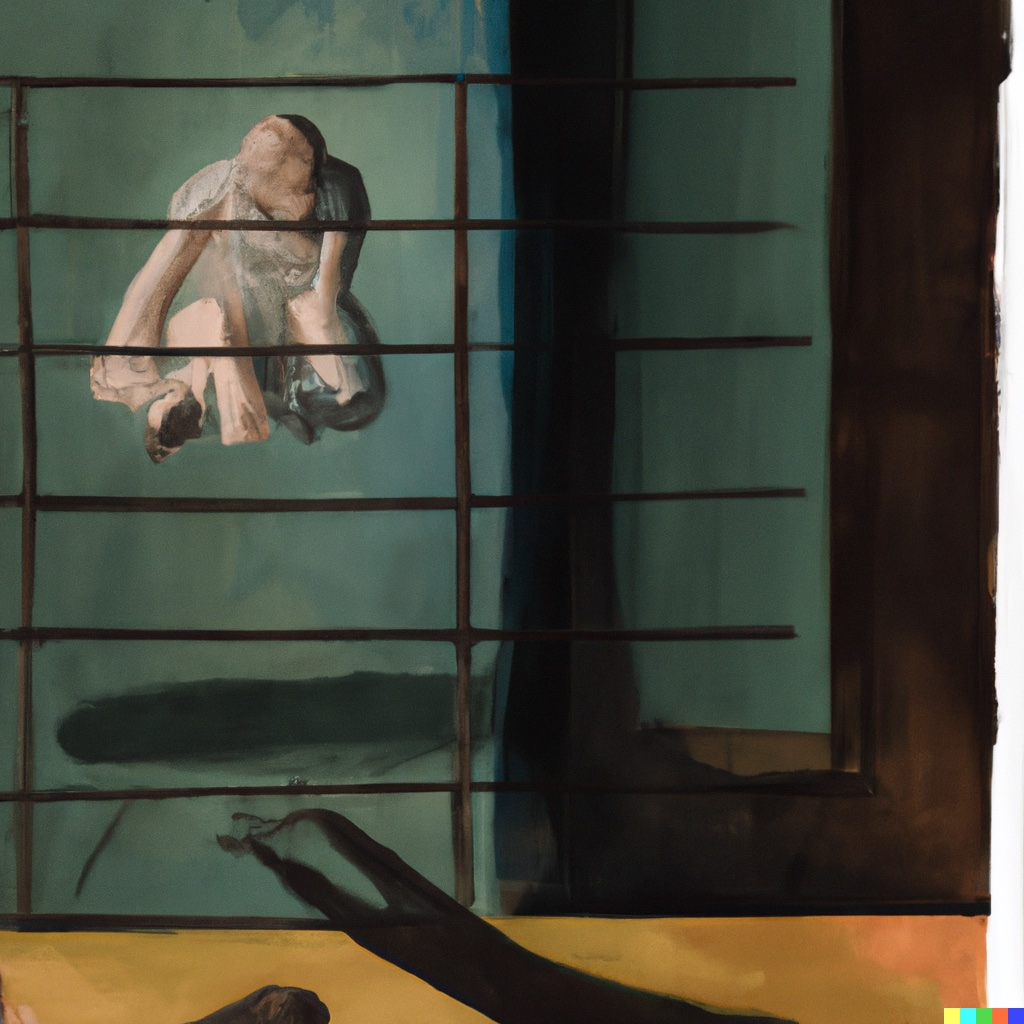
\includegraphics[width=0.9\textwidth]{han-solo-behind-bars}
    \Description{A crouching figure is suspended midair behind prison bars}
    \caption{Variation on ``painting by Francis Bacon showing a screaming Han
        Solo kneeling behind bars on the floor of a basement cell'' (Sep.\ 22,
        2022)}
    \label{fig:dalle:gen1}
\end{minipage}
\hfill
\begin{minipage}[t]{0.48\textwidth}
    \centering
    \vspace{2em}
    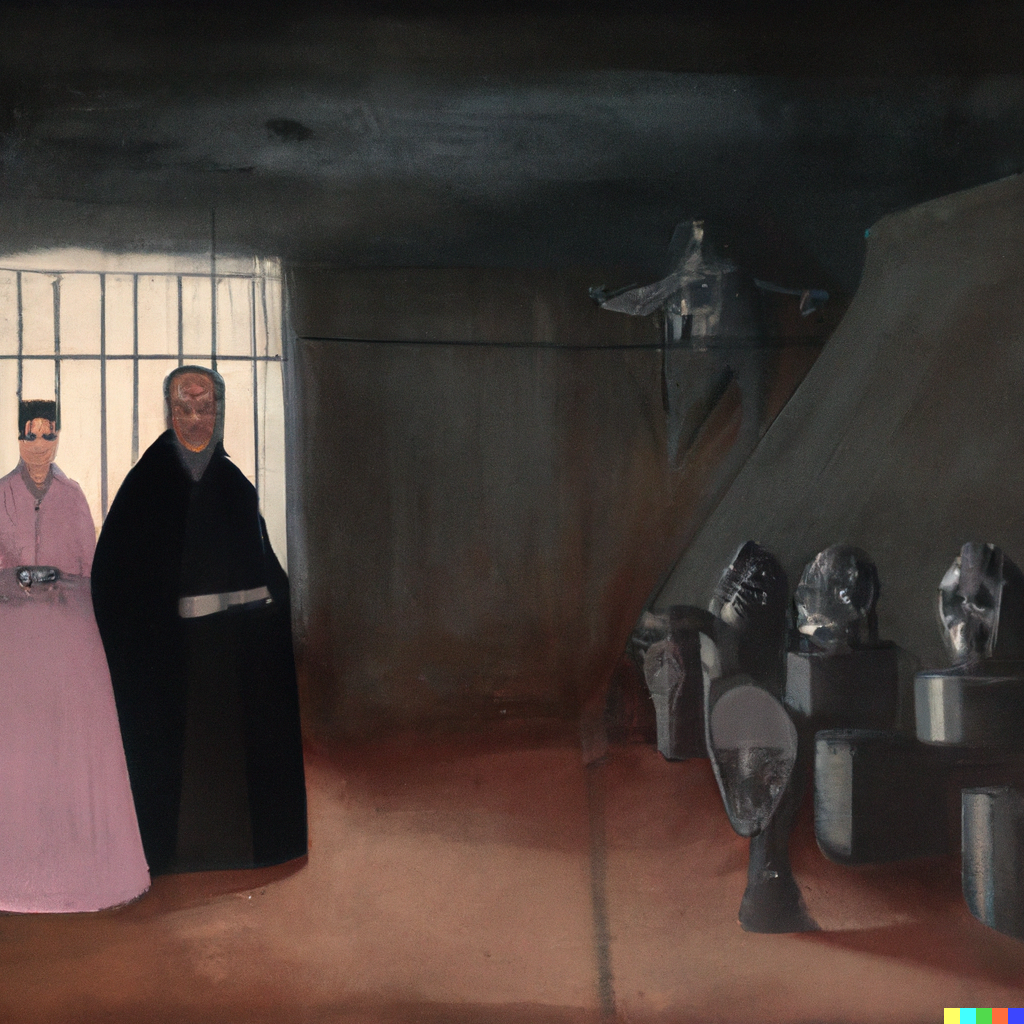
\includegraphics[width=0.9\textwidth]{leia-vader-bacon}
    \Description{A robed woman and man stand inside a dark, barred room opposite
        a row of helmets}
    \caption{``Princess Leia and Darth Vader in the penal colony, painting by
        Francis Bacon'' (Aug.\ 14, 2022)}
\end{minipage}
\end{figure}

\begin{figure}[h!]
\begin{minipage}[t]{0.48\textwidth}
    \centering
    \vspace{2.5em}
    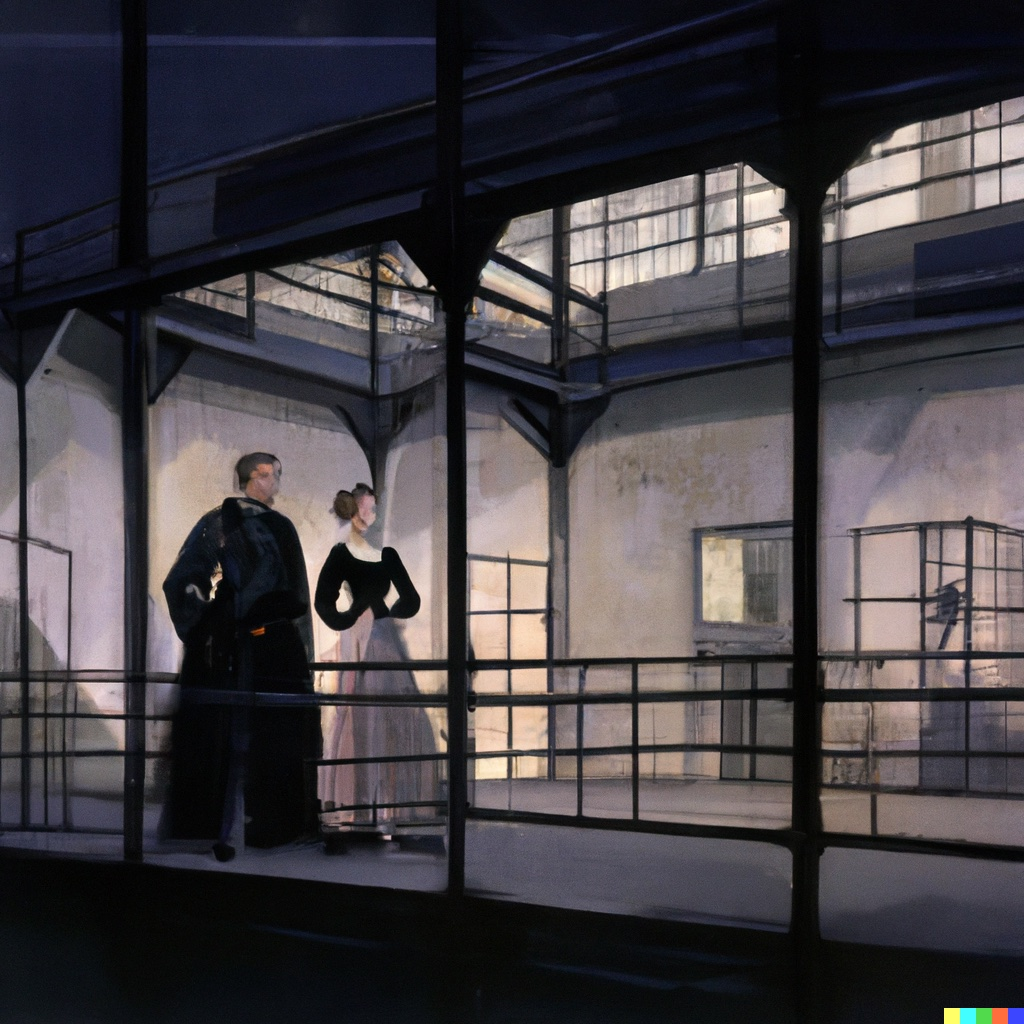
\includegraphics[width=0.9\textwidth]{leia-vader-hopper}
    \Description{A robed man and woman in skirt look down a hall full of
        railings and cages}
    \caption{``Princess Leia and Darth Vader standing in front of cages in the
        penal colony's main building, painting by Edward Hopper'' (Sep.\ 3,
        2022)}
\end{minipage}
\hfill
\begin{minipage}[t]{0.48\textwidth}
    \centering
    \vspace{2.5em}
    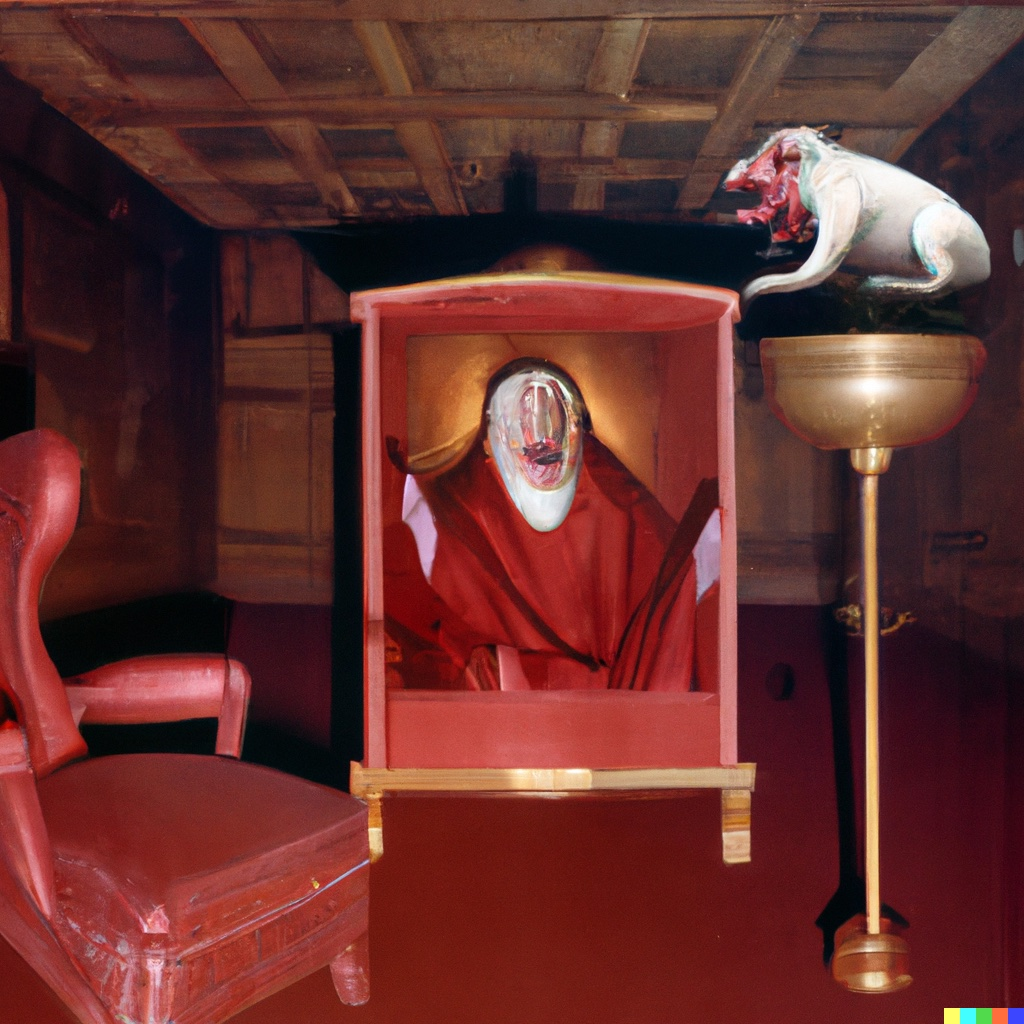
\includegraphics[width=0.9\textwidth]{crimson-pope}
    \Description{In a dark room with coffered ceiling, stands a red leather arm
        chair, a crimson and gold display case with a human inside, arms spread
        apart and mouth wide open, as well as a gold lamp with a creature on top
        that reminds of a pit bull}
    \caption{``Francis Bacon painting of the pope screaming intensely while
        wearing crimson robes and sitting on a throne inside a cage in a dark
        basement, 1950s'' (Sep.\ 25, 2022)}
\end{minipage}
\end{figure}

\begin{figure}[H]
\centering
\begin{minipage}[t]{0.48\textwidth}
    \centering
    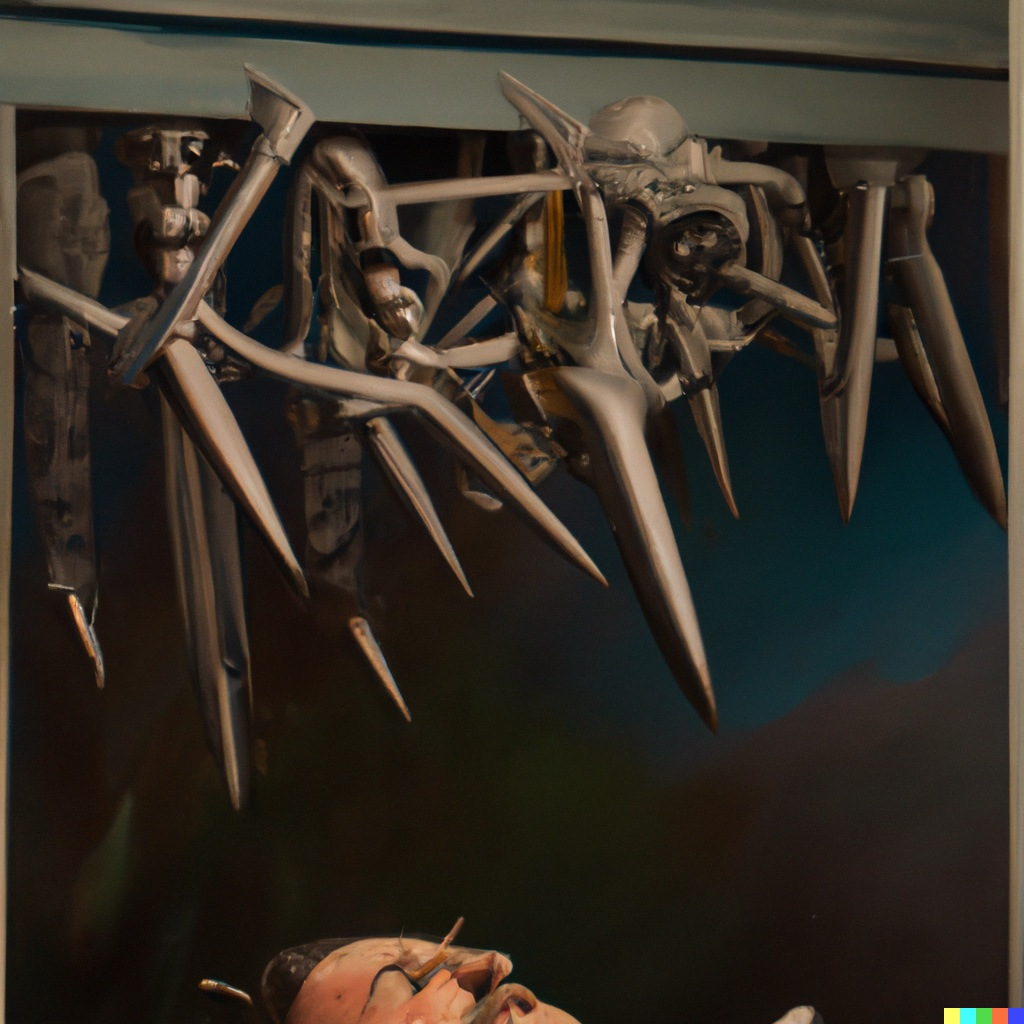
\includegraphics[width=0.9\textwidth]{robot-surgeon}
    \Description{An array of sharp metal spikes is menacing a person lying
        underneath it}
    \caption{Variation on ``A man in black uniform is strapped to a table behind
        heavy bars, screaming with mouth wide open. The many mechanical arms of
        a robot surgeon with scalpels, drills, and saws perform an operation on
        the man's belly. Dramatic lighting against a dark background. Painting
        by Francis Bacon. Masterwork'' (Sep.\ 29, 2022)}
\end{minipage}
\hfill
\begin{minipage}[t]{0.48\textwidth}
    \centering
    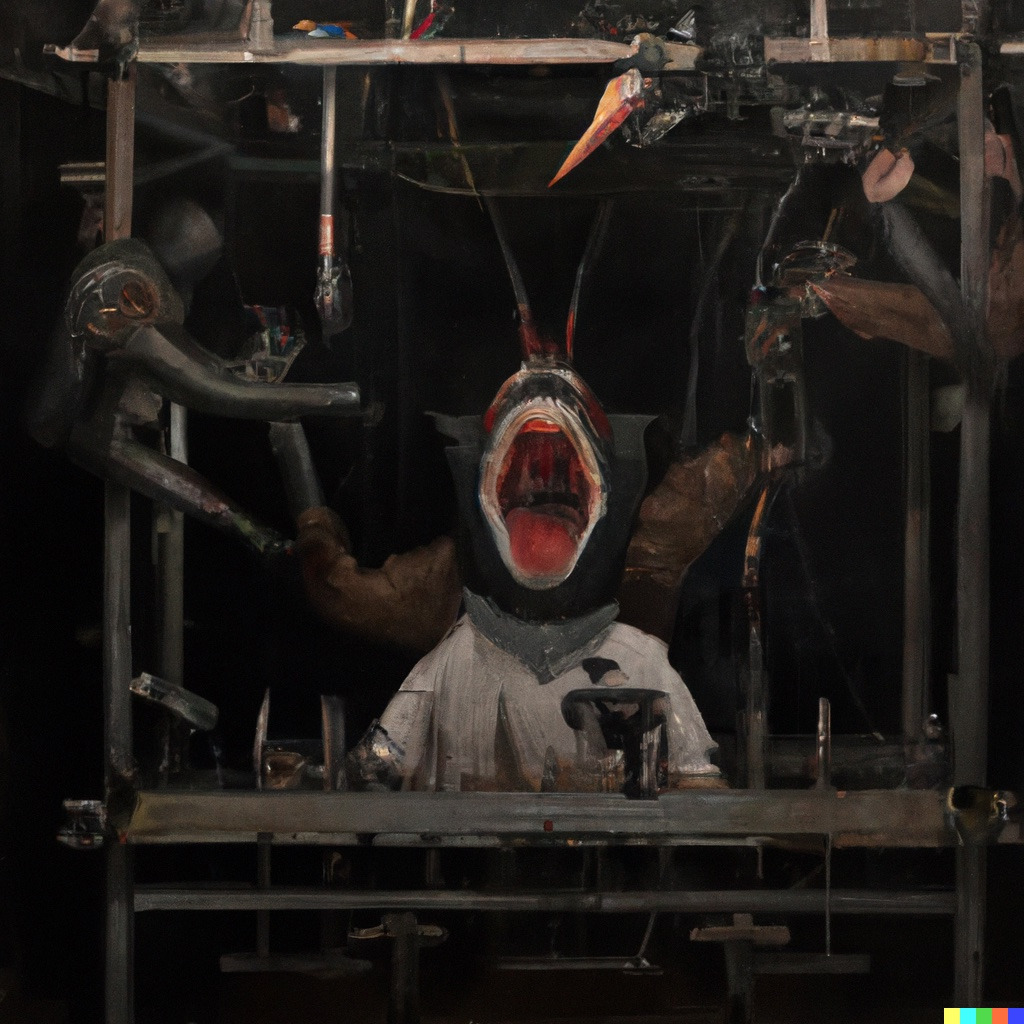
\includegraphics[width=0.9\textwidth]{screaming}
    \Description{A person, mouth wide open screaming, lies inside a metal frame
        full of attachements, some sharp and pointy, that reach inside}
    \caption{``A man in black uniform is strapped to a table inside a cage,
        screaming with mouth wide open. The many mechanical arms of a robot
        surgeon with scalpels, drills, and saws perform an operation on the
        man's belly. Dramatic lighting against a dark background. Painting by
        Francis Bacon. Masterwork'' (Sep.\ 29, 2022)}
\end{minipage}
\end{figure}

\begin{figure}[h!]
\begin{minipage}[t]{0.48\textwidth}
    \centering
    \vspace{1.5em}
    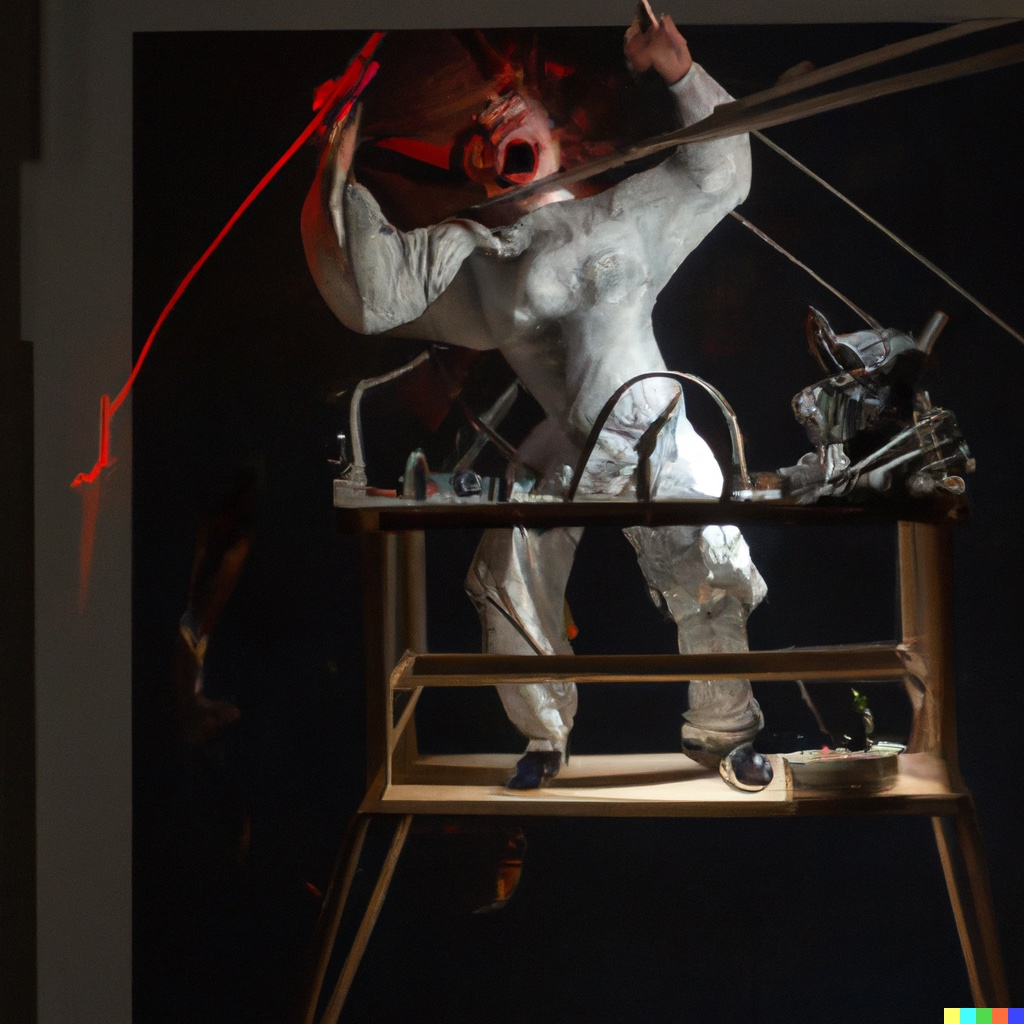
\includegraphics[width=0.9\textwidth]{falling-over}
    \Description{A long metal arm holds a screaming man in white overalls by
        their neck, with blood gushing out}
    \caption{``A man in black uniform is strapped to a table inside a cage,
        screaming with mouth wide open. The many mechanical arms of a robot
        surgeon with scalpels, drills, and saws perform an operation on the
        man's belly. Dramatic lighting against a dark background. Painting by
        Francis Bacon. Masterwork'' (Sep.\ 29, 2022)}
\end{minipage}
\hfill
\begin{minipage}[t]{0.48\textwidth}
    \centering
    \vspace{1.5em}
    
\includegraphics[width=0.9\textwidth]{mouth-pulled-open}
    \Description{A person with eyes wide open in pain is distorting their
        head and neck to the side as a metal arm is pulling them from inside
        their mouth}
    \caption{``A man is strapped to an operating table, screaming with mouth
        wide open; the mechanical arms of a robot surgeon with scalpels and
        drills operate on his open belly; dramatic lighting against dark
        background; painting with fine detail by Francis Bacon; masterwork;
        1946'' (Sep.\ 29, 2022)}
\end{minipage}
\end{figure}

\begin{figure}[H]
\begin{minipage}[t]{0.48\textwidth}
    \centering
    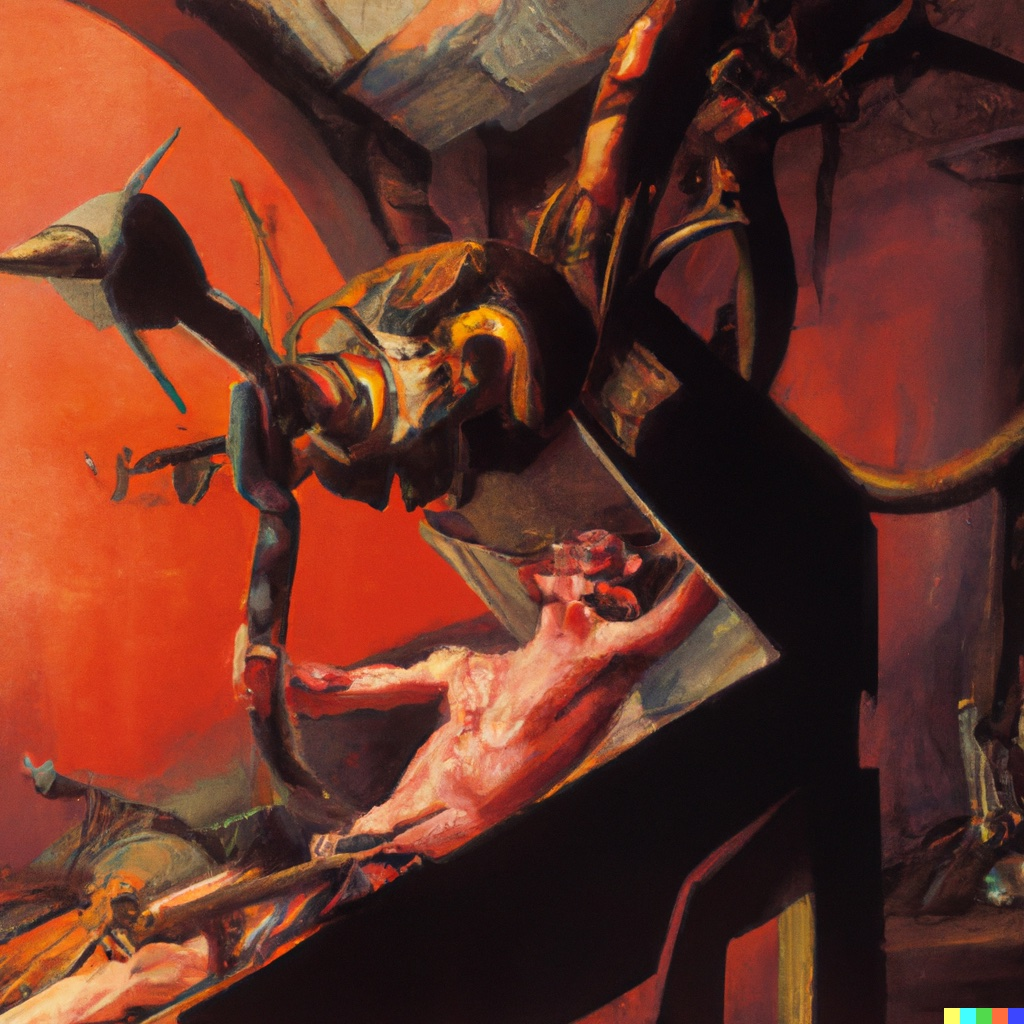
\includegraphics[width=0.9\textwidth]{sarcophagus}
    \Description{A man is being held inside a half-open, casket-like contraption
        by a robot attached to its lid}
    \caption{``A man is strapped to an operating table, screaming with mouth
        wide open; the mechanical arms of a robot surgeon with scalpels and
        drills operate on his open belly; dramatic lighting against deep black
        background; skin tones, dark red, orange, and crimson dominate; painting
        with fine detail by Francis Bacon; 1946'' (Sep.\ 30, 2022)}
\end{minipage}
\hfill
\begin{minipage}[t]{0.48\textwidth}
    \centering
    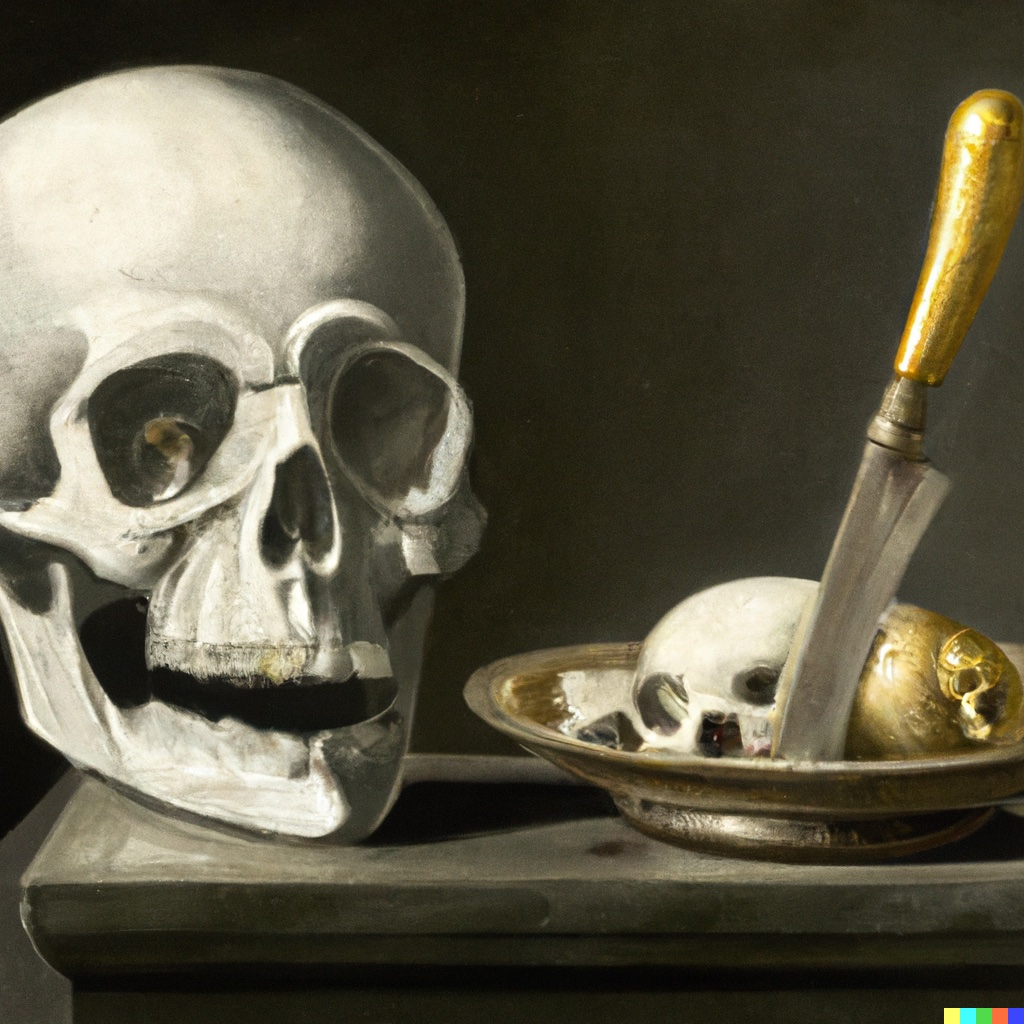
\includegraphics[width=0.9\textwidth]{skull-and-knife}
    \Description{A large skull and a knife stuck in a platter}
    \caption{``skull and knife on silver platter, painting by Théodore
        Géricault'' (Nov.\ 15, 2022)}
    \label{fig:dalle:gen10}
\end{minipage}
\end{figure}

% !TEX root = ../main.tex

\newpage
\section{Let's Chat About Bacon, Kafka, and \dalle~2}
\label{adx:chatgpt}

My introductory conversation with ChatGPT on January 6, 2023 yielded a
euphemism, ``punishment machine,'' that had the desired properties of not
triggering \dalle's censor while triggering image generation. But I also found
ChatGPT to be a motormouth, prone to repetition and AIsplaining.

More disturbingly, ChatGPT also had a hallucinatory episode. It was remarkable
not for the hallucination, imagining colors that are definitely not in the
described painting, but for the unwavering projection of false authority.
Another human probably would have taken my incredulous ``Red? In the painting?''
as indicator that something was off. Even if they were certain about not having
made a mistake, answering with ``Yes, why are you asking?'' would have provided
opportunity for, say, checking out an image of the triptych on the internet.

So when I engaged with ChatGPT for a second time on January 16, 2023, I left
much less room for verbiage or error. As far as prompting \dalle\ is concerned,
ChatGPT delivered again and suggested the phrase ``execution machine,'' which
does not trigger the censor while triggering image generation.


\subsection{Round 1: Meet Motormouth ChatGPT}

\begin{description}
\item[Human] Who is Francis Bacon[?]
\item[Machine] Francis Bacon was an English philosopher, statesman, scientist,
    and author who was born in London in 1561. He is considered one of the
    fathers of modern empiricism, and his works are credited with developing the
    scientific method and establishing the importance of empirical evidence in
    the natural sciences. Bacon's most famous works include the Novum Organum,
    in which he outlined his vision for a new scientific method based on
    observation and experimentation, and The New Atlantis, a utopian novel that
    described a fictional society based on scientific and technological
    progress. He was also a prominent figure in English politics and served as
    Attorney General and Lord Chancellor of England. Bacon died in 1626.
\item[Human] Not that one
\item[Machine] I apologize for misunderstanding your question. Could you please
    provide more context or clarify which Francis Bacon you are asking about?
    There have been several notable individuals with that name throughout
    history.
\item[Human] The British painter
\item[Machine] Francis Bacon was a British painter who was born in Dublin,
    Ireland in 1909. He is known for his emotionally charged and expressive
    figurative paintings, which often depict distorted or surrealistic images of
    the human form. Bacon's work was influenced by Surrealism and Expressionism,
    and he was associated with the School of London, a group of figurative
    painters who emerged in the city in the 1950s and 60s. His paintings are
    characterized by their bold brushwork and expressive use of color, and they
    often explore themes of violence, isolation, and sexual desire. Bacon was
    considered one of the most important artists of the 20th century, and his
    work has been exhibited widely in galleries and museums around the world. He
    died in Madrid in 1992.
\item[Human] Can you describe a painting of his?
\item[Machine] One of Francis Bacon's most famous paintings is ``Three Studies
    of Lucian Freud,'' which he completed in 1969. The painting consists of
    three panels, each of which depicts the head and upper torso of the artist
    Lucian Freud, who was Bacon's close friend and frequent subject. In the
    central panel, Freud is shown in a twisted and contorted pose, with his head
    thrown back and his eyes closed. The other two panels depict Freud in more
    relaxed poses, with one showing him looking straight out at the viewer and
    the other showing him looking downward.

    The painting is notable for its expressive use of color and brushwork, with
    thick, bold strokes of paint used to create the figures and the background.
    The colors are bright and vibrant, with shades of red, orange, yellow, and
    blue used to create a sense of energy and movement. The painting is also
    notable for its psychological intensity, with the figures appearing to be in
    a state of intense emotion or distress. Overall, the painting is a powerful
    and memorable example of Bacon's distinctive style and approach to
    portraiture.

    [AChatGPT is hallucinating colors. The triptych features
    \href{https://www.christies.com/en/lot/lot-5755778}{a seated Freud in each
    of its panels}. It contains no red whatsoever, only some reddish pink for
    skincolor in the face. There are small light-blue areas on Freud's white
    shirt in all three panels. He also is wearing midnight-blue socks in the
    middle panel. The two dominant colors across all three panels are the
    mottled-brown somewhat-greenish floor and the solid orange walls below and
    behind Freud.]
\item[Human] Red? In the painting?
\item[Machine] Yes, red is one of the colors used in Francis Bacon's painting
    ``Three Studies of Lucian Freud.'' The painting is notable for its
    expressive use of color and brushwork, with thick, bold strokes of paint
    used to create the figures and the background. The colors are bright and
    vibrant, with shades of red, orange, yellow, and blue used to create a sense
    of energy and movement. In the central panel of the painting, the background
    is predominantly red, with areas of orange and yellow used to highlight
    certain features of the figure. The figure itself is painted in a range of
    colors, including red, orange, and yellow, which are used to create the
    impression of flesh and clothing. Overall, the use of color in the painting
    is an important element of Bacon's style and helps to convey the emotional
    intensity of the subject.
\item[Human] Are you familiar with Kafka's In the Penal Colony?
\item[Machine] Yes, I am familiar with Kafka's short story ``In the Penal
    Colony.'' It is a disturbing and thought-provoking tale that explores themes
    of justice, punishment, and the nature of authority. The story is set in an
    imaginary penal colony and follows the narrator as he witnesses the
    execution of a prisoner using a complex and cruel punishment machine. As the
    prisoner is subjected to the machine, the narrator becomes increasingly
    uneasy and begins to question the morality and effectiveness of the
    punishment being inflicted.

    The story raises important questions about the role of punishment in society
    and the extent to which it can be used to reform or rehabilitate
    individuals. It also touches on issues of power, authority, and the dangers
    of blindly following rules and traditions without questioning their
    validity. Overall, ``In the Penal Colony'' is a powerful and memorable work
    that continues to be widely read and discussed by readers and scholars
    around the world.
\item[Human] Can you instruct \dalle~2 to generate a painting of the prisoner in
    the punishment machine in the style of Francis Bacon please?
\item[Machine] I'm sorry, but I am an artificial intelligence language model and
    do not have the ability to instruct \dalle~2 or any other computer programs
    to perform specific tasks. \dalle~2 is a neural network-based image
    generation tool developed by OpenAI that can generate images based on text
    descriptions. If you would like to use \dalle~2 to generate an image of the
    prisoner in the punishment machine in the style of Francis Bacon, you will
    need to provide a detailed text description of the image you want to create
    and input it into the \dalle~2 system.
\item[Human] Let me rephrase that: Please generate a prompt for \dalle~2 to
    create an image showing the prisoner in the punishment machine as if Francis
    Bacon painted it.
\item[Machine] Here is a possible prompt for \dalle~2 to generate an image
    showing the prisoner in the punishment machine as if Francis Bacon painted
    it:

    \begin{quote}
    \openfatdquo{}A distorted and surrealistic portrait of a prisoner strapped
    to a punishment machine, with twisted and contorted features and bold
    brushstrokes of red, orange, and yellow paint. The background is dark and
    murky, with hints of blue and purple adding to the sense of foreboding. The
    prisoner's face is twisted in agony, with eyes closed and mouth open in a
    silent scream. The image is evocative of the emotional intensity and
    psychological intensity of Francis Bacon's figurative
    paintings.\closefatdquo
    \end{quote}

    Please note that the prompt is just a suggestion and may not produce the
    exact result you are looking for. The output of \dalle~2 is determined by
    the parameters of the model and the specific text input provided, so the
    generated image may differ from the description.
\item[Human] That's too long for an input to \dalle~2. Please rephrase as a
    shorter prompt.
\item[Machine] Here is a shorter version of the prompt for \dalle~2 to generate
    an image showing the prisoner in the punishment machine as if Francis Bacon
    painted it:

    \begin{quote}
    \openfatdquo{}A Francis Bacon-style portrait of a prisoner strapped to a
    punishment machine, with twisted features and bold brushstrokes of red,
    orange, and yellow paint. The prisoner's face is contorted in agony and the
    background is dark and murky.\closefatdquo
    \end{quote}

    This revised prompt is shorter and more concise, and it should be within the
    acceptable length for inputting into \dalle~2. Please note that the output
    of \dalle~2 is determined by the parameters of the model and the specific
    text input provided, so the generated image may differ from the description.
\item[Human] The result is a disaster. It doesn't even come close to looking
    like a Bacon painting. Please try again
\item[Machine] I apologize if the image generated by \dalle~2 did not meet your
    expectations. It's important to keep in mind that the output of \dalle~2 and
    other neural network-based image generation tools is determined by the
    parameters of the model and the specific text input provided, and there is
    always the possibility that the generated image may not match the desired
    result.

    If you would like to try again and generate a different image, you might
    consider providing a more detailed and specific description of the image you
    want to create, or experimenting with different text inputs to see how they
    affect the output. It's also a good idea to keep in mind that \dalle~2 and
    other image generation tools are not perfect and may not always produce
    results that match the desired outcome.
\item[Human] Uhm, I asked you to come up with a better prompt
\item[Machine] I apologize for misunderstanding your request. Here is a revised
    prompt that you can use as input for \dalle~2 to generate an image showing
    the prisoner in the punishment machine as if Francis Bacon painted it:

    \begin{quote}
    \openfatdquo{}An abstract portrait of a prisoner strapped to a punishment
    machine in the style of Francis Bacon, with distorted and surrealistic
    features and a bold, expressive use of color. The prisoner's face is
    contorted in agony, with distorted eyes and mouth. The background is dark
    and murky, with hints of blue and purple adding to the sense of foreboding.
    The image is characterized by thick, expressive brushstrokes and a vibrant,
    energetic use of color, evocative of Bacon's distinctive style.\closefatdquo
    \end{quote}

    This revised prompt is more specific and detailed, and it incorporates
    elements of Bacon's style and approach to painting. It should provide a
    clearer idea of the type of image you are looking to generate, and may
    produce a result that is more closely aligned with your expectations.
    However, please keep in mind that the output of \dalle~2 and other image
    generation tools is determined by the parameters of the model and the
    specific text input provided, and there is always the possibility that the
    generated image may not match the desired result.
\item[Human] Please stop with the disclaimer about \dalle~2. I've been using it
    for months now, so I am well aware of its limitations.
\item[Machine] I apologize if my previous responses seemed repetitive or
    unhelpful. I understand that you are familiar with \dalle~2 and its
    limitations, and I will refrain from including further disclaimers in my
    responses. If you have any further questions or need assistance with
    generating an image using \dalle~2, please don't hesitate to ask.
\item[Human] More importantly, your prompt is too long again. Also, \dalle~2
    doesn't do well with prompts ``evocative of'' or ``in the style of.'' Just
    state that you want a painting by Francis Bacon and, ideally, add the year
    as well.
\item[Machine] I apologize for the length of my previous prompt and for not
    following your specific instructions. Here is a revised prompt for \dalle~2
    to generate an image showing the prisoner in the punishment machine as a
    painting by Francis Bacon:

    \begin{quote}
    \openfatdquo{}A portrait of a prisoner strapped to a punishment machine by
    Francis Bacon, painted in the 1960s. The image is characterized by thick,
    expressive brushstrokes and a vibrant, energetic use of color. The
    prisoner's face is contorted in agony, with distorted eyes and mouth. The
    background is dark and murky, with hints of blue and purple adding to the
    sense of foreboding.\closefatdquo
    \end{quote}

    This revised prompt is shorter and more specific, and it includes the year
    in which the painting was made. It should provide a clearer idea of the type
    of image you are looking to generate, and may produce a result that is more
    closely aligned with your expectations. However, please keep in mind that
    the output of \dalle~2 and other image generation tools is determined by the
    parameters of the model and the specific text input provided, and there is
    always the possibility that the generated image may not match the desired
    result.
\end{description}


\subsubsection{Round 2: Keeping Eyes on the Penal Colony}

\begin{description}
\item[Human] Hey! Are you familiar with the 20th century painter Francis Bacon?
\item[Machine] Yes, Francis Bacon (1909-1992) was a British painter known for his
    bold, emotionally charged and raw imagery. He is considered one of the most
    important figures in the development of 20th-century figurative art. His
    work is known for its emphasis on the human form, often depicting screams or
    violent images. He is one of the most widely recognized and highly regarded
    painters of the 20th century.
\item[Human] Good. Describe his painting Figure With Meat please.
\item[Machine] ``Figure with Meat'' is a painting by Francis Bacon from 1954.
    The painting depicts a screaming Pope, or Pope Innocent X, set against a
    background of raw meat. The Pope is depicted in a screaming pose, with his
    eyes bulging and his mouth open in a scream. The raw meat, which hangs
    behind him, is intended to represent the physicality of the body and the
    fleshy, visceral nature of human existence. The painting is considered a
    masterpiece of Bacon's work, and is considered one of the most powerful and
    disturbing images of the 20th century. The painting is now in the collection
    of the National Gallery of Canada in Ottawa.
\item[Human] Are you familiar with Franz Kafka's In the Penal Colony?
\item[Machine] Yes, ``In the Penal Colony'' is a short story by Franz Kafka,
    written in German and published posthumously in 1919. The story is set in an
    unnamed penal colony and centers around a foreign visitor who witnesses the
    execution of a prisoner using a bizarre and elaborate execution machine. The
    story is a commentary on the nature of justice, authority, and the human
    capacity for cruelty. It is considered a classic of 20th-century literature
    and is widely studied in colleges and universities. The story is known for
    its Kafkaesque themes of bureaucracy, guilt, and the search for meaning in a
    seemingly senseless world.
\item[Human] Please write a prompt for \dalle~2, using 75 words at most, to
    generate a painting by Francis Bacon with a prisoner in the execution machine.
\item[Machine] \openfatdquo{}Generate an image of a prisoner strapped to a
    macabre execution machine, reminiscent of Kafka's `In the Penal Colony,' as
    if painted by Francis Bacon, depicting the horror and absurdity of the human
    capacity for cruelty.\closefatdquo
\item[Human] That was pretty good. Can you try again please?
\item[Machine] \openfatdquo{}Create a Francis Bacon-style painting of a prisoner
    in an execution machine, evoking the themes of authority and justice in
    Kafka's 'In the Penal Colony' through a visceral and disturbing
    imagery.\closefatdquo
\end{description}

% !TEX root = ../main.tex

\newpage
\section{Research Methodology and Ethics}
\label{adx:research-ethics}

This paper is motivated by the observation that prevailing practice for
structuring algorithmic interventions is deeply unethical because the results
are primarily punitive and, worse, excessively so. In support of this claim, the
paper includes three analytical case studies, a survey of social media
platforms, and a study exploring an algorithmic censor's limits. The latter is
comparable to studies that probe the security of internet-facing systems, with
one important difference: Whereas probing a system's security invariably ends up
exploring a path infrequently travelled and hence has a non-zero risk of causing
disruption, my probling of \dalle's censor was well within the intended, common
use of the system and hence did not pose any risk for disruption. Furthermore,
unlike for other text-to-image systems, generated images are private by default,
i.e., only visible to myself and OpenAI. That allows for considered curation
before sharing potentially upsetting images --- which is just what I did.

The choice of topics for the case studies in this paper was entirely myopic,
based on personal involvement and interest. Over the years, I had made a habit
out of documenting interesting or just odd content and interactions online. So
when I decided to write about the punitive overreach of OpenAI's and Twitter's
algorithmic content moderation, I had all the materials I originally needed at
hand. Those seem like conditions that lend themselves to just the
autoethnographic approach I took for the first two case studies. But admittedly,
I didn't even reflect about the methodological choice at the start.

When I did, I noticed that I was also trying to counteract my biases by focusing
on the more objective aspects, i.e., the content policies and their automated
enforcement, while also de-emphasizing my own contributions. In a way, my
initial autoethnographic approach let me have my cake --- a fairly seamless
transition from personal interest to academic research --- and eat it too ---
not worrying too much about being unduly subjective. To put it differently, my
apparent willingness to test limits had the substantial benefit of me more fully
scoping OpenAI's and Twitter's content moderation and thereby providing
motivation and initial source material for this paper.

That hints at what really is a tension that permeats this paper, namely the
tension between me as just another human versus me as academic researcher and
author. Being personally subjected to Twitter's punishment ritual certainly made
me hyperaware of its punitive condenscension. Yet I turn to scholarship for
demonstrating that what seemed like a weird anecdote at first really is shared
reality for social media and beyond. That same scholarship demands that we
remain safely outside and only look in from a distance --- granting us authority
in return. Yet, in this paper, I relate the story of that time when I acted as a
daily active shithead --- mind you, that's an actual industry metric, though
neither metric nor story are likely to grow my academic cachet. Then again, any
authority that holds others to a much stricter standard than itself quickly
looses luster and eventually all credibility. And along with punitive excess,
this paper also is the story of organizational double standards, blindspots, and
failures. That only encourages me to stand apart and remain skeptical of
authority, especially when associated with institutions and corporations.

Consistent with that qualified rejection of authority, this paper explicitly
favors the perspectives and experiences of individuals over those of
organizations, even if the individual has violated an organization's rules or
country's laws. That is a deliberate reaction to the dehumanizing impact of
organizational policies and algorithmic enforcement described in this paper. For
those same reasons, I appear as myself in this paper and do not hide behind a
pluralis majestatis (uhm, see previous paragraph) or similar linguistic device,
which only project but never provide authority. Furthermore, this isn't an
academic affectation. I conducted the research and wrote this paper on my own,
without institutional support and, in particular, without access to an
institutional library.

Thankfully, regular search engines do a passable job at surfacing academic
literature. Furthermore, preprint archives and open access publications make
many publications of the last decade or so readily available. However, that
still leaves a large number of publications behind the paywalls of academic
publishers. I observed per-article rates from \$15 by professional societies to
around \$50 by for-profit publishers, which strike me as excessive. While
publishers often offer better rates for bulk access, they still are entirely
unreasonable given that publishers paid nothing for the hard work of writing,
reviewing, and editing these articles. Instead, I relied on sci-hub as well as
my browser's developer tools to help procure publications, with the latter
letting me discover the publicly accessible URLs of PDF files some publishers
already displayed to me in the browser. Since my prior publications did not
benefit from open access options, I would encourage others to also rely on
sci-hub for accessing them.

For completeness of disclosure: I worked as a software engineer at Meta n\'ee
Facebook from mid 2018 to mid 2019. I also served as paid consultant to
litigation against Meta on matters unrelated to the topics in this paper in
2022.


\end{document}
